\documentclass[12pt]{article}
\usepackage{graphicx,xr}
\usepackage{setspace}
%\DeclareGraphicsExtensions{.eps, .ps}
\usepackage{soul,color}
\usepackage{amsmath,amsthm,amsfonts}
\usepackage{newfloat}
\usepackage{multirow}
\usepackage{arydshln,hyperref}
\usepackage[authoryear]{natbib}
\bibliographystyle{plainnat}

\usepackage[margin = 1in]{geometry}
\usepackage{setspace}
%\onehalfspacing
\doublespacing

\makeatletter
\newcommand*{\addFileDependency}[1]{% argument=file name and extension
  \typeout{(#1)}
  \@addtofilelist{#1}
  \IfFileExists{#1}{}{\typeout{No file #1.}}
}
\makeatother

\newcommand*{\myexternaldocument}[1]{%
    \externaldocument{#1}%
    \addFileDependency{#1.tex}%
    \addFileDependency{#1.aux}%
}

% put all the external documents here!
\myexternaldocument{./main-supp}

%\startlocaldefs

\def\pr{\text{pr}}
\def\E{\mathbb{E}}
\def\P{\mathbb{P}}
\def\given{\, | \,}
\def\Ep{\E_{\bf p}}
\def\Eeta{\E_{\eta}}
\def\U{\mathcal{U}}
\def\V{\mathcal{V}}

% \font\fiverm=cmr5
% \arraycolsep=1pt

\newtheorem{thm}{Theorem}[section]
\newtheorem{lemma}[thm]{Lemma}
\newtheorem{prop}[thm]{Proposition}
\newtheorem{cor}[thm]{Corollary}
\newtheorem{defn}[thm]{Definition}
\newtheorem{example}[thm]{Example}
\newtheorem{conj}[thm]{Conjecture}
\newtheorem{assumption}[thm]{Assumption}
\newtheorem{principle}[thm]{Principle}
\newtheorem{observation}[thm]{Observation}
\newtheorem{remark}[thm]{Remark}%\endlocaldefs

%% ZW commands
\newcommand{\zw}[1]{\textcolor{blue}{[\textit{ZW: #1}]}}
%% HS commands
\newcommand{\hs}[3]{\textcolor{red}{[\textit{HS: #1}]}}



\begin{document}
\title{Assessing Time-Varying Causal Effect Moderation in the Presence of Cluster-Level Treatment Effect Heterogeneity}
\author{Jieru Shi, Zhenke Wu, Walter Dempsey}
\maketitle
\begin{abstract}\noindent
% Advances in mobile devices and wearable sensors have enabled the delivery of behavioral treatments in the users natural environment, helping to support behavior change and maintenance.

The micro-randomized trial (MRT) is a sequential randomized experimental design to empirically evaluate the effectiveness of mobile health (mHealth) intervention components that may be delivered at hundreds or thousands of decision points. The MRT context has motivated a new class of causal estimands, termed ``causal excursion effects", for which inference can be made by a weighted, centered least squares approach (Boruvka et al., 2017). Existing methods assume between-subject independence and non-interference. Deviations from these assumptions often occur which, if unaccounted for, may result in bias and overconfident variance estimates. In this paper, causal excursion effects are considered under potential cluster-level correlation and interference and when the treatment effect of interest depends on cluster-level moderators. The utility of our proposed methods is shown by analyzing data from a multi-institution cohort of first year medical residents in the United States. The approach paves the way for construction of mHealth interventions that account for observed social network information.
\end{abstract}

\noindent {\it Keywords:} Causal Inference; Clustered Data; Just-In-Time Adaptive Interventions; Microrandomized Trials; Mobile Health; Moderation Effect

\section{Introduction}

In many areas of behavioral science, push notifications in mobile apps that are adapted to continuously collected information on an individual's current context have received a considerable amount of attention.  These time-varying adaptive interventions are hypothesized to lead to meaningful short- and long-term behavior change. The assessment of the time-varying effect of such push notifications motivated sequential randomized designs such as the micro-randomized trial (MRT) \citep{Nahum2017, KlasnjaMRT}. In an MRT, interventions are randomized to be potentially delivered at hundreds or thousands of decision points. The MRT design enables the estimation of the time-delayed marginal treatment effects of a push notification upon the outcome of interest at multiple time-lags, referred to as ``causal excursion effects" \citep{Boruvkaetal, Qian2021}. A weighted, centered least squares (WCLS) approach has been developed to consistently estimate causal excursion effects with robust methods of uncertainty assessment. Extensions to balance the number of randomizations by observed or derived individual-level contextual information have also been developed, e.g., a stratified MRT~\citep{DempseyAOAS}.

Existing inferential methods for data collected in an MRT rely on two key assumptions. First, an intervention delivered to an individual is assumed to only impact the outcome of that individual, i.e., non-interference. Second, the method assumes no stochastic dependence among outcomes of different subjects. Deviations from these assumptions, however, may occur when individuals naturally form clusters.  Consider, for example, an MRT in which medical interns are recruited from several institutions and every week potentially receive push notifications designed to improve physical activity, mood, or sleep. First, \textit{interference} may occur when an intern receiving a push notification to increase their steps may then encourage another intern in the same specialty and institution to do the same hence altering the others' outcomes. Second, even if there is no direct interference, interns in the same specialty and institution are likely to have correlated outcomes, induced by variation in unobserved factors shared within each cluster. For example, interns within a specialty and institution may share similar experiences during their residency which will lead to a higher correlation in their weekly mood scores than interns in different specialties or institutions.

The primary contribution of this paper is the significant extension of data analytic methods for MRTs to account for potential cluster-level correlation and the extension of the causal excursion effect to account for potential interference, i.e., we define both a direct and indirect causal excursion effect.  In Section~\ref{section:preliminaries}, we review the MRT design and the existing method's implicit assumptions.  In Section~\ref{section:cond_effects}, we introduce the moderated causal excursion effect using a cluster-based conceptualization of potential outcomes \citep{Hong2006,Vanderweele2013}.  We then generalize the WCLS criterion to a cluster-based WCLS (C-WCLS) criterion to estimate both direct and indirect causal excursion effects in Section~\ref{section:estimation}.  Finally, we demonstrate that when proximal outcomes exhibit within-cluster correlation but there is an absence of between-cluster treatment effect heterogeneity, our proposal agrees with the traditional approach both in terms of the point estimate and the asymptotic variance.  In Section~\ref{section:casestudy}, we illustrate the proposed method by estimating the causal excursion effects of push notifications on mood, sleep, and step count for a cohort of first year medical residents in the United States. The paper concludes with a brief discussion.

\section{Preliminaries}
\label{section:preliminaries}

We first review the design of MRTs and the existing inferential methods based on MRT data. We focus on the assumptions made in the inferential methods to set the stage for our proposed extension.

\subsection{Micro-Randomized Trials (MRT)}

An MRT consists of a sequence of within-subject decision times $t=1,\ldots,T$ at which treatment options may be randomly assigned.  The resulting longitudinal data for any subject can be summarized as
$$
\{ O_0, O_1, A_1, O_2, A_2, \ldots, O_T, A_T, O_{T+1} \}
$$
where $t$ indexes a sequence of decision points, $O_0$ is the baseline information, $O_t$ is the information collected between time $t-1$ and $t$ which may include mobile sensor and wearable data, and $A_t$ is the treatment option provided at time $t$.  In an MRT, $A_t$ results from randomization at each decision point; here, we assume this randomization probability depends on the complete observed history $H_t := \{ O_0, O_1, A_1, \ldots, A_{t-1}, O_t \}$ and is denoted $p_t (A_t \given H_t)$. Treatment options are designed to impact a proximal response $Y_{t+1}$ which is a known function of $\{ O_t, A_t, O_{t+1}\}$.
% \zw{An example for $Y_{t+1}$ as a function of $A_t$? Are you thinking about interference? }  \wd{This is to mimic rewards from RL where you can change reward to depend on actions (e.g., utility defn).  Avoided going into it but can if you think it's critical}
In this section, we will use HeartSteps~\citep{HeartSteps2018}, an MRT designed to increase physical activity among sedentary adults, as our illustrative example.
In~HeartSteps~\citep{HeartSteps2018},  $A_t = 1$ denotes sending a tailored activity message designed to increase proximal physical activity and therefore $Y_{t+1}$ is chosen to be total step count in the 30-minutes after the decision time.

\begin{remark} \normalfont
At some decision points, it is inappropriate for scientific, ethical, or burden reasons to provide treatment. To address this, the observation vector $O_t$ also contains an indicator of availability:
$I_t = 1$ if available for treatment and $I_t = 0$ otherwise. Availability at time $t$ is determined before treatment randomization. When an individual is unavailable for treatment ($I_t = 0$), then no treatment is provided ($A_t = 0$). In this paper, for simplicity, individuals are assumed always available for treatment. All methods can be readily extended to account for availability as in \citet{Boruvkaetal}.

% Estimands need only condition on availability, i.e., $I_t = 1$, while least squares criterion need only multiply each decision point specific weight by $I_t$.

% \zw{Perhaps provide a rationale for why this extension is straightforward, e.g., same estimand, or different estimand?}
\end{remark}

\subsection{Estimand and Inferential Method}
\label{section:standardmrtmethods}

Following \cite{Boruvkaetal}, \cite{Qian2021}, and \cite{DempseyAOAS}, we focus on the class of estimands that is referred to as ``causal excursion effects" defined by
$$
\beta (t;s) = \E \left[ \E \left[ Y_{t+1} \given H_t, A_t = 1 \right] - \E \left[ Y_{t+1} \given H_t, A_t = 0 \right] \given S_t = s\right]
$$
where $S_t$ is a time-varying potential effect moderator (or ``state") and a deterministic function of the observed history $H_t$. For example, in the HeartSteps study, $S_t$ may represent subject-specific contextual information such as step count in the previous 30 minutes.
% \textcolor{red}{An estimate of the moderation effect by $S_t$ may reveal treatment effect heterogeneity for subjects with distinct values of $S_t$.}
See Section \ref{section:prox_effects_pot_outcome} for how this estimand is derived using potential outcomes.  Under the assumption that $\beta(t;s) = f_t(s)^\top \beta^\star$ where $f_t(s) \in \mathbb{R}^q$ is a feature vector depending only on state $s$ and decision point $t$, a consistent estimator $\hat \beta$ can be obtained by minimizing the following weighted and centered least squares (WCLS) criterion:
\begin{equation}
\label{eq:mrtstandard}
\arg \min_{\alpha, \beta} \mathbb{P}_n \left[ \sum_{t=1}^T W_t \left( Y_{t+1} - g_t(H_t)^\prime \alpha - (A_t - \tilde p_t (1 \mid S_t)) f_t (S_t)^\top \beta \right)^2 \right]
\end{equation}
where~$\mathbb{P}_n$ is defined as the average of a function over the sample, $W_t = \tilde p_t (A_t \mid S_t) / p_t (A_t \mid H_t)$ is a weight where the numerator is an arbitrary function with range $(0,1)$ that only depends on $S_t$ and the denominator is the MRT specified randomization probability, and $g_t(H_t) \in \mathbb{R}^p$ are a set of control variables chosen to help reduce the variance of the estimators and to construct more powerful test statistics. In HeartSteps, for example, a natural control variable is the number of steps in the prior 30 minutes as this variable is likely highly correlated with the proximal response and thus can be used to reduce variance in the estimation of $\beta$. See~\cite{Boruvkaetal} for additional details on how to define and estimate moderated time-varying treatment effects using data from an MRT.

\section{Cluster-Level Proximal Treatment Effects}
\label{section:cond_effects}

MRTs are implicitly defined with the individual as the unit of analysis.  The associated analytics rely on statistical independence among individuals in deriving asymptotic normality; moreover, the treatment effects assume that treatments provided to one individual do not impact another individual. In Section~\ref{section:sims}, we show that the nominal coverage probability of the $95\%$ confidence interval obtained from these methods decays quickly when the MRT is conducted among individuals with cluster-level treatment effect heterogeneity.  Moreover, in such a setting, an interesting scientific question concerns moderation analysis where the moderator is defined at the cluster-level, i.e., average values of a moderator such as mood or step-count across a cluster.
% \zw{add an example of such moderators.}
Here we consider a cluster-based definition of causal excursion effect and corresponding analyses to address these issues. We start with our motivating example that demonstrates the necessity for considering clustering in the context of MRTs.

\subsection{Motivating Example}
\label{section:motex}

The Intern Health Study (IHS) is a 6-month micro-randomized trial on 1,565 medical interns~\citep{Necamp2020}.  Due to high depression rates and levels of stress during the first year of physician residency training, a critical question is whether targeted notifications can be used at the right time to improve mood, increase sleep time, and/or increase physical activity. Enrolled medical interns were randomized weekly to receive either mood, activity, or sleep notifications or receive no notifications for that week (probability 1/4 each).  On a week in which notifications are provided, interns were randomized daily to receive a notification with probability 50\%. Hence for a notification week, the user received, on average, 3.5 notifications. The exploratory and MRT analyses conducted in this paper focus on weekly randomization; See~\cite{Necamp2020} for further study details.

Medical internships occur in a specific location and within a specific specialty.  The 1,565 interns in the MRT represented 321 different residency locations and 42 specialties.  Thus, interns are naturally clustered.  Table~\ref{tab:IHSanova} presents a standard equally-weighted analysis of variance (ANOVA) applied to the average weekly mood scores with three factors: week-in-study, residency and specialty both interacted with weekly treatment (Txt). Compared with the residual mean square of 1.27, there is considerable excess variation associated with week-in-study (28.44), residency by treatment (5.89) and specialty by treatment (8.41). In other words, the ANOVA suggests proximal responses exhibit potential within-cluster correlation within residency locations and specialties that varies with treatment. In this paper, we focus on defining clusters using specialty and institution information and do not discuss multi-level clusters.

\begin{table}[!th]
\centering
\begin{tabular}{l | rrr}
Source & d.f. & Sum Sq. & Mean Sq. \\ \hline
week-in-study & 25 & 711 & 28.44 \\
Residency:Txt & 1091 & 6424 & 5.89 \\
Specialty:Txt & 48 & 404 & 8.41 \\
Residuals & 38946 & 49479 & 1.27 \\ \hline
\end{tabular}
\label{tab:IHSanova}
\caption{ANOVA decomposition for average weekly mood scores in the IHS.}
\end{table}

Three immediate questions may arise:
\begin{itemize}
    \item[(1)] Does the standard MRT analysis still have good statistical properties, e.g., consistency and valid nominal coverage probability of $95\%$ confidence intervals, when participants exhibit within-cluster correlation?
    \item[(2)] Can one assess potential cluster-level effect moderators using the standard MRT analysis? and,
    \item[(3)] Can one extend the MRT analysis to assess the effect of treatment provided to one individual on the proximal response of another individual in the same cluster?
\end{itemize}
  For (1), through a simulation study in Section~\ref{section:sims}, we demonstrate potential deficiency of the standard WCLS method that results in severe under-coverage of nominal $95\%$ confidence intervals. In particular, we use simulation settings that mimic realistic cluster-level treatment heterogeneity.  For (2), in IHS, for example, a scientific question may be how group average mood impacts the proximal effect of notifications on average daily mood.  Since each individual's mood may be impacted by their own treatments, if the proximal effect is moderated by cluster-level summary variables then this implies the proximal response is a function of past treatment assignment to all individuals in the group.  Finally, for (3), in Section~\ref{section:prox_effects_pot_outcome} we extend the causal excursion effect to distinguish between direct and indirect causal excursion effects.

In this paper, we extend WCLS method \citep{Boruvkaetal} to  account for clustered continuous outcomes and potential within-cluster interference of other subjects' treatments upon one subject's outcome, offering a general framework for answering the three questions above. Here we study micro-randomized trials in which there is a pre-defined cluster-level structure.  The cluster structure may result in (A) within-cluster correlation among proximal responses (question 1), (B) treatment impacting individual-level moderators which then impact proximal responses of other individuals (question 2), or (C) treatment interference, i.e., treatment provided to one individual may impact the proximal response of another individual in the same cluster (question 3).  We will demonstrate how our proposed method addresses these three issues.


\subsection{Proximal Moderated Treatment Effects}
\label{section:prox_effects_pot_outcome}

The primary question of interest is whether the treatment has a proximal effect. Here, potential outcomes are used to define the proximal effects. Due to potential treatment interference in the cluster MRT setting, we consider two types of moderated effects: a direct and an indirect effect, both on the linear scale.

Consider a cluster of size $G$.  The overbar is used to denote a sequence through a specified treatment occasion; $\bar a_{t,j} = (a_{1,j},\ldots, a_{t,j})$, for instance, denotes the sequence of realized treatments up to and including decision time $t$ for individual $j \in [G]:=\{1,\ldots, G\}$ in the cluster.   Let $\bar a_{t} = (\bar a_{t,1}, \ldots, \bar a_{t,G})$ denote the set of realized treatments up to and including decision time $t$ for all individuals in the cluster and $\bar a_{t,-j} = \bar a_t \backslash \bar a_{t,j}$ to denote this set with the $j$th individual's realized treatments removed. Let $Y_{t+1,j} (\bar a_{t})$ denote the potential outcome for individual $j \in [G]$ in the cluster.  Note that the potential outcome for individual $j$ may depend on the realized treatments for all members in the cluster.
% and that cluster-size may vary.
% \zw{cluster sizes may differ}

\noindent \textbf{Direct causal effects}.
In standard MRTs, the individual is the unit of interest.  In our current setting, the cluster is the unit of interest.  At the cluster level, our interest lies in the effect of providing treatment versus not providing treatment at time $t$ on a random individual in the group.  This can be expressed as a difference in potential outcomes for the proximal response and is given by
\begin{equation}
\label{eq:directeffect}
\frac{1}{G} \sum_{j=1}^G \left[ Y_{t+1,j} (\bar a_{t,-j}, (\bar a_{t-1,j}, a_{t,j}=1)) - Y_{t+1,j} (\bar a_{t,-j}, (\bar a_{t-1,j}, a_{t,j}=0)) \right].
\end{equation}
Equation~\eqref{eq:directeffect} is a \emph{direct causal effect} of treatment compared to no treatment on the proximal response for the same individual, while all previous treatments on the individual and all treatments on every other member of the cluster are fixed to specific values.
% \zw{clarify the directness means blocking all other paths except the path from $A_{tj}$ to $Y_{t+1,j}$}

The ``fundamental problem of causal inference''~\citep{Rubin, Pearl2009} is that these individual differences cannot be observed. Thus, similar to prior work~\citep{DempseyAOAS, Boruvkaetal}, in this paper averages of potential outcomes are considered in defining treatment effects. Let $S_t (\bar a_{t-1})$ denote a vector of potential moderator variables chosen from $H_t (\bar a_{t-1})$, the \emph{cluster-level} history up to decision point $t$.  We write $S_t (\bar a_{t-1}) = \left( S_{t,j} (\bar a_{t-1}), S_{t,-j} (\bar a_{t-1}) \right)$ to clarify that the potential moderator variables can contain both information on the selected individual as well as other individuals in the cluster. Then moderated direct treatment effect, denoted $\beta (t; s)$, can be defined as
\begin{equation}
\label{eq:directavglineareffect}
\begin{array}{r@{}l}
\mathbb{E} \bigg[ Y_{t+1,J} &(\bar A_{t,-J}, (\bar A_{t-1,J}, 1)) \\
- &Y_{t+1,J} (\bar A_{t,-J}, (\bar A_{t-1,J}, 0)) \mid \left( S_{t,J} (\bar A_{t-1}), S_{t,-J} (\bar A_{t-1}) \right) = (s_J, s_{-J}) \bigg].
\end{array}
\end{equation}
where $J$ is a uniformly distributed random index defined on $[G]$. The expectation is over both the potential outcomes~($Y_{t+1,J}(\cdot)$), the set of randomized treatments~($\bar A_{t,-J}$ and $\bar A_{t-1,J}$), and the random index~($J$).
% \zw{Perhaps can talk about the expectation is over both Y and A; and write it in a way that addresses potential issues that may be raised by the utility of this estimand and how is it different from existing ones.}  \wd{Now raising the expectations point but pushing discussion of the estimand and its difference from other stuff to that 3.2.3 section}
Different choices of variables in $S_t (\bar A_{t-1})$ address a variety of scientific questions.  A primary analysis, for instance, may focus on the marginal proximal effects and therefore set $S_t (\bar A_{t-1}) = \emptyset$.  A second analysis may focus on assessing the effect conditional on variables only related to the individual indexed by $J$ and set $S_t (\bar A_{t-1}) = X_{t,J} (\bar A_{t-1,J})$, where $X_{t,J} (\bar A_{t-1,J}) \subset O_{t,H} (\bar A_{t-1,J})$ is a potential moderator of interest.  A third analysis may consider moderation by the average value across all individuals $S_t (\bar A_{t-1}) = G^{-1} \sum_j X_{t,j} (\bar A_{t-1,j})$ or the joint moderation of the individual's mood and the average of the other individuals' moods $S_t (\bar A_{t-1}) = \left( X_{t,j}(\bar A_{t-1,j}), \frac{1}{G-1} \sum_{j^\prime \neq j} X_{t,j^\prime} (\bar A_{t-1,j^\prime}) \right)$.


\noindent \textbf{Indirect causal effects}.
Of secondary interest is the effect of providing treatment versus not providing treatment to the $j$th individual at time $t$ on a different individual's proximal response when they do not receive treatment, i.e., within-cluster treatment interference.  This \emph{indirect causal effect} is given by
\begin{align}
\frac{1}{G \cdot (G-1)} \sum_{j^\prime \neq j}& \left[Y_{t+1,j} (\bar a_{t,-\{j, j^\prime\}}, (\bar a_{t-1,j}, a_{t,j}=0), (\bar a_{t-1,j^\prime}, a_{t,j'}=1)) \right.\nonumber\\
& ~~~~ - \left.Y_{t+1,j} (\bar a_{t,-\{j, j^\prime\}}, (\bar a_{t-1,j}, a_{t,j}=0), (\bar a_{t-1,j^\prime}, a_{t,j'}=0))\nonumber \right].
\end{align}
Again, since the individual differences cannot be observed, we consider averages of potential outcomes in defining indirect treatment effects. The moderated indirect treatment effect, denoted $\beta^{(IE)} (t; s)$, can be defined by
\begin{equation}
\label{eq:inddirectavglineareffect}
\begin{array}{r@{}l}
\mathbb{E} \bigg[ Y_{t+1,J} (\bar A_{t,-\{J, J^\prime\}}, &(\bar A_{t-1,J}, 0), (\bar A_{t-1,J^\prime}, 1)) \\
&- Y_{t+1,J} (\bar A_{t,-\{J, J^\prime\}}, (\bar A_{t-1,J}, 0), (\bar A_{t-1,J^\prime}, 0)) \mid S_t (\bar A_{t-1}) \bigg].
\end{array}
\end{equation}
where $J^\prime$ is uniformly distributed random index on the set $[G] \backslash \{J\}$. The expectation is again over both the potential outcomes~($Y_{t+1,J}(\cdot)$), the set of randomized treatments~($\bar A_{t,-\{J,J^\prime\}}$, $\bar A_{t-1,J}$, and $\bar A_{t-1,J^\prime}$), and the random indices~($J$ and $J^\prime$). Here, the potential moderator can be written as $S_t (\bar A_{t-1}) = \left( S_{t,J} (\bar A_{t-1}), S_{t,J^\prime} (\bar A_{t-1}), S_{t,-\{J, J^\prime \}} (\bar A_{t-1}) \right)$ to clarify that the variables can contain both information on the two selected individuals as well as others in the cluster. Note that a similar effect can be defined when the individual does receive treatment. For now, we focus on the effect defined by~\eqref{eq:inddirectavglineareffect}.

% \subsubsection{Total causal effects (necessary?)}


\subsection{Estimand Dependence on Treatment Distribution}

It is useful to distinguish the above estimands, the traditional MRT estimand~\citep{Boruvkaetal}, and estimands commonly studies in longitudinal treatment effect estimation~\citep{Robins}. In the causal inference literature, the typical estimand is an expected outcome for a particular sequence of treatments,i.e.,~$\E \left[ Y(a_1,\ldots, a_T)\right]$.  Such estimands do not depend on the treatment distribution, but are often not of primary interest in the current MRT setting since many sequences of treatment may never be observed in finite samples given the large number of decision points (often hundreds or thousands).

The estimands considered in this paper are most similar to average outcomes under a particular dynamic treatment regime~$\E_\pi \left[ Y(A_1,\ldots, A_T)\right]$ where $\pi$ denotes the dynamic treatment regime from which the treatments are drawn~\citep{MurphyJASA2001}. Indeed, for any $A_{u,j}$ not contained in $S_t (\bar A_{t-1})$, the direct and indirect effects depend on the distribution of $\{ A_{u,j} \}_{u < t, j \in [G]}$.  Estimands~\eqref{eq:directeffect} and~\eqref{eq:inddirectavglineareffect} marginalize over treatments not contained in $S_t(\bar A_{t-1})$ under the micro-randomized distribution.  Marginalization over different probabilistic assignment of treatments may yield different results. Therefore, the marginal direct and indirect effects depend on the study protocol. The reason for this is that micro-randomization is meant to gather information on how to optimize the design of intervention components~\citep{Collins2018}.  The marginal formulation of main and moderation effects characterizes contrasts excursions from the current treatment proctocol, mimics analyses used in a factorial design that marginalize over factors including time. See~\citet[Section 8]{Qian2021} for additional considerations.  Regardless, the effects considered in this paper are causal and depend on the cluster-level treatment distribution.  Due to this dependence, we recommend presenting the micro-randomization distribution together with the estimated treatment effects.

\subsection{Proximal Effect of Treatment \& Observable data: Identification}
\label{section:prox_effects_data}
Causal effects \eqref{eq:directavglineareffect} and~\eqref{eq:inddirectavglineareffect} can be expressed in terms of the observable data under the following standard set of causal inference assumptions~\cite{Robins}:

\begin{assumption} \normalfont
  \label{consistency}
  We assume consistency, positivity, and sequential ignorability:
  \begin{itemize}
  \item Consistency: For each~$t \leq T$ and $j \in [G]$,
    $\{Y_{t+1,j} (\bar{A}_{t} ), O_{t,j} (\bar A_{t-1}), A_{t,j} (\bar{A}_{t-1} )\}  = \{Y_{t+1, j}, O_{t,j}, A_{t,j}\}$.
    That is, the observed values equal the corresponding potential outcomes;
  \item Positivity: if the joint density~$\{ H_t = h, A_t = a\}$ is greater
    than zero, then~$\mathbb{P} (A_t = a_t \given H_t = h_t ) > 0$;
  \item Sequential ignorability: for each~$t \leq T$, the
    potential outcomes,\\ $\{Y_{2,j} ( a_{1}), O_{2,j}(a_{1}),A_{2,j}( a_{1}), \ldots,
    Y_{T,j} (\bar a_{T-1}) \}_{j \in [G], \bar a_{T-1}\in \{0,1\}^{(T-1)\times G}}$, are independent of~$A_{t,j}$ conditional on the observed history~$H_t$.
  \end{itemize}
\end{assumption}

Sequential ignorability and, assuming all of the randomization probabilities are bounded away from $0$ and $1$, positivity, are guaranteed in our setting  by design. In a standard MRT, the randomization probabilities may depend on the individual's observed history so $\Pr(A_t = a_t \mid H_t = h_t) = \prod_{j=1}^G \Pr(A_{t,j} = a_{t,j} \mid H_{t,j} = h_{t,j})$ and the positivity constraint can be placed on the individual-level randomization probabilities.  Here, we allow for the possibility that the randomization probabilities depend on the cluster-level history. Consistency is a necessary assumption for linking the potential outcomes as defined here to the data. Since an individual's outcomes may be influenced by the treatments provided to other individuals in the same cluster, consistency holds due to our use of a cluster-based conceptualization of potential outcomes as seen in~\cite{Hong2006} and \cite{Vanderweele2013}.

\begin{lemma}
  \label{lemma:cond_effect}
  Under assumption~\ref{consistency}, the moderated direct treatment effect~$\beta(t;s)$ is equal to
  $$
  \mathbb{E} \left[ \frac{1}{G} \sum_{j=1}^G \mathbb{E} \left[ Y_{t+1,j} \mid H_{t}, A_{t,j} = 1 \right] - \mathbb{E} \left[ Y_{t+1,j} \mid H_{t}, A_{t,j} = 0 \right] \mid S_t \right]
  $$
  where each expectation is with respect to the distribution of the
  data collected using the treatment assignment probabilities. Under assumption~\ref{consistency}, the moderated indirect treatment effect~$\beta(t;s)^{(IE)}$ is equal to
  $$
  \mathbb{E} \left[ \frac{1}{G (G-1)} \sum_{j \neq j^\prime} \mathbb{E} \left[ Y_{t+1,j} \mid H_{t}, A_{t,j} = 0, A_{t,j^\prime} = 1 \right] - \mathbb{E} \left[ Y_{t+1,j} \mid H_{t}, A_{t,j} = 0, A_{t,j^\prime} = 0 \right] \mid S_t \right].
  $$
\end{lemma}
\noindent Proof of Lemma~\ref{lemma:cond_effect} can be found in the Appendix~\ref{app:techdetails}.

\section{Estimation}
\label{section:estimation}

In this section, we consider estimation of the two estimands defined in Lemma~\ref{lemma:cond_effect} using cluster MRT data.

\subsection{Direct Effect Estimation}
We make the following assumptions regarding the direct treatment effect specification:

\begin{assumption} \normalfont
\label{ass:directeffect}
Assume the treatment effect,~$\beta(t;S_t)$, of interest satisfies
$$
\E \left[ \E \left[ Y_{t+1, J} \mid H_t, A_{t,J} = 1 \right] - \E \left[ Y_{t+1, J} \mid H_t, A_{t,J} = 1 \right] \mid S_t \right] = f_t (S_t)^\top \beta^\star
$$
where $f_t (s) \in \mathbb{R}^p$ is a $p$-dimensional vector function of $s$ and time $t$.
\end{assumption}

We now consider inference on the unknown $p$-dimensional parameter $\beta^\star$. To do so, we define the weight~$W_{t,j}$ at decision time $t$ for the $j$th individual as equal to $\frac{\tilde p (A_{t,j} \mid S_t)}{p_t (A_{t,j} \mid H_t)}$ where $\tilde p_t (a \mid S_t)\in (0,1)$ is arbitrary as long as it does not depend on terms in $H_t$ other than $S_t$, and $p(A_{t,j} \mid H_t)$ is the marginal probability that individual $j$ receives treatment $A_{t,j}$ given $H_t$.  For now, we consider pre-specified $\tilde p_t (a \mid S_t)$  (i.e., does not depend on the observed MRT data). Here we consider an estimator~$\hat \beta$ of $\beta^\star$ which is the minimizer of the following cluster-based,  weighted-centered least-squares (C-WCLS) criterion, minimized over $(\alpha, \beta)$:
\begin{equation}
\label{eq:directwcls}
\mathbb{P}_M \left[ \frac{1}{G_m} \sum_{j=1}^{G_m} \sum_{t=1}^T W_{t,j} \left(Y_{t+1,j} - g_t (H_t)^\prime \alpha - (A_{t,j} - \tilde p_t (A_{t,j} \mid S_t)) f_t(S_t)^\top \beta \right)^2 \right]
\end{equation}
where $\mathbb{P}_M$ is defined as the average of a function over the sample, which in this context is the sample of \emph{clusters} rather than the sample of \emph{individuals} as in traditional MRT settings. In Appendix~\ref{app:techdetails}, we prove the following result.

\begin{lemma}
\label{lemma:asymnorm}
Under assumption~\ref{ass:directeffect}, given invertibility and moment conditions, the estimator $\hat \beta$ that minimizes \eqref{eq:directwcls} satisfies $\sqrt{M} \left(\hat \beta - \beta^\star \right) \to N(0, Q^{-1} W Q^{-1})$ where
$$
Q = \mathbb{E} \left[ \sum_{t=1}^T \tilde p_t( 1 \mid S_{t} ) ( 1- \tilde p_t( 1 \mid S_{t} )) f_t (S_t) f_t (S_t)^\top \right]
$$
and
$$
W =  \mathbb{E} \left[ \sum_{t=1}^T W_{t,J} \, \epsilon_{t,J} ( A_{t,J} - \tilde p_t( 1 \mid S_{t} )) f_t (S_t) \times \sum_{t=1}^T W_{t, \tilde J} \, \epsilon_{t, \tilde J} ( A_{t, \tilde J} - \tilde p_t( 1 \mid S_{t} )) f_t (S_t)^\top  \right]
$$
% \zw{Should the second sum over t inside E be deleted?}: Both sums should be inside
where $\epsilon_{t,j} = Y_{t+1, j} - g_t(H_t)^\prime \alpha^\star - (A_{t,j} - \tilde p_t (1 \mid S_t) ) f_t (S_t)^\top \beta^\star$, $\alpha^\star$ minimizes the least-squares criterion $\mathbb{E}  \left[G^{-1} \sum_{j=1}^G \sum_{t=1}^T W_{t,j} \left( Y_{t+1,j} - g_t(H_t)^\prime \alpha \right)^2 \right]$, and both $J$ and $\tilde J$ are independent randomly sampled indices from the cluster.
\end{lemma}

\noindent In practice, plug-in estimates $\hat Q$ and $\hat W$ are used to estimate the covariance structure. Appendix~\ref{app:ssa} presents small sample size adjustments that we use in simulation and analysis in this paper.  It is clear that from Lemma~\ref{lemma:asymnorm} that use of standard MRT data analytic methods, i.e., equation~\eqref{eq:mrtstandard}, will produce biased estimates for the marginal effect of interest if cluster size is variable.

\begin{remark}[$L_2$ Projection interpretation]
\label{rmk:l2proj}
\normalfont
Importantly, Assumption~\ref{ass:directeffect} is not required.  That is, we can follow~\cite{Neugebauer2007,Rosenblum2010,Kennedy2019,DempseyAOAS} and others in using $f_t (S_t)^\top \beta$ as a working model.  Specifically, instead of making the strong modeling assumption as in~\cite{Boruvkaetal}, the estimate~$\hat \beta$ can be considered a consistent estimator of a parameter $\beta^\star$ which is a solution to the following weighted least squares projection
$$
\beta^\star = \arg \min_{\beta} \mathbb{E} \left[ \frac{1}{G} \sum_{j=1}^G \sum_{t=1}^T \tilde p_t(1 \mid S_t) \left( 1 - \tilde p_t(1 \mid S_t) \right) \left( \beta(t; S_t) - f_t (S_t)^\top \beta \right)^2 \right].
$$
Here, the weight is the variance of the numerator in the weight~$W_{t,j}$.  To interpret as a projection or to make the stronger Assumption~\ref{ass:directeffect} can be viewed as a bias-variance trade-off.  The projection interpretation guarantees well-defined parameter interpretation in practice where Assumption~\ref{ass:directeffect} is unlikely to hold.  See~\cite[Sec. 3.1, pp.9--10]{Kennedy2019} for a great discussion of the use of in causal versus predictive settings.
\end{remark}

\subsubsection{Connection To A Semiparametric Efficient Estimator}

A special case of both effects is when $S_t$ is set to the observed history~$H_t$.  In this case, estimators for this fully conditional case can be derived based on semiparametric efficiency theory~\citep{Newey1990,Tsiatis2007} under a lack of interference assumption.

\begin{lemma}
Under the semiparametric model~\eqref{ass:directeffect}, Assumptions~\ref{consistency}, and the stronger \emph{lack of interference} assumption, the semiparametric efficient score for $\beta$ is
\begin{equation}
\label{eq:effscore}
S_{\text{eff}} (\beta) = \frac{1}{G} \sum_{j=1}^G \sum_{t=1}^T (Y_{t+1,j} - \mu (H_{t,j}) - (A_{t,j} - p_t (1 \mid H_{t,j})) f_t (H_{t,j})^\top \beta ) K_{t,j} (A_{t,j} - p_t(1 \mid H_{t,j})) f(H_{t,j})
\end{equation}
where
\begin{align*}
\mu_t (H_{t,j}) = \mathbb{E} &\left[ Y_{t+1,j} \mid H_{t,j} \right], \quad \text{and} \quad \sigma^2_{t+1} (H_{t,j}, A_{t,j}) = \text{Var} \left( Y_{t+1,j} \mid H_{t,j}, A_{t,j} \right) \\
K_{t,j} = &\bigg[ \frac{1}{\sigma^2_{t+1,j} (H_{t,j}, 1)} + p_t ( 1 \mid H_{t,j}) \left[  \frac{p_t (1 \mid H_{t,j} )}{\sigma^2_{t+1,j} (H_{t,j}, 1)} + \frac{1-p_t (1 \mid H_{t,j} )}{\sigma^2_{t+1,j} (H_{t,j}, 0)} \right] \times \\
&\left( \frac{1}{\sigma^2_{t+1,j} (H_{t,j}, 1)}  - \frac{1}{\sigma^2_{t+1,j} (H_{t,j}, 0)} \right)
 \bigg]
\end{align*}
\end{lemma}

Semiparametric efficiency theory states that the solution $\hat \beta$ to $\mathbb{P}_n S_{\text{eff}} (\psi) = 0$ achieves the semiparametric efficiency bound~\citep{Newey1990}. \cite{Qian2021} proved a similar result for the causal excursion effect on the relative risk scale for binary outcomes.  Unlike~\cite{Qian2021}, the efficient score here requires estimates of the conditional variance, which may be difficult to obtain. Corollary~\eqref{cor:semiparametricconnection} motivates the C-WCLS criterion for the direct effect given by~\eqref{eq:directwcls} from the semiparametric efficiency perspective under particular working homoskedastic assumptions on the conditional variance~$\sigma^2_{t+1} (H_{t,j}, A_{t,j})$ and a working model~$g_t (H_{t,j})^\prime \alpha$ for the unknown quantity~$\mu(H_{t,j})$.  Making the homoskedastic assumption helps avoid the conditional variance estimation problem.  While this establishes a connection between the C-WCLS criterion and semiparametric efficiency scores, more work on efficiency theory for causal excursions effects is considered important future work.

\begin{cor}
\label{cor:semiparametricconnection}
Under the assumption $\text{Var}(Y_{t+1,j} \mid H_{t,j}, A_{t,j}) := \sigma^2_{t+1}(H_{t,j})$,i.e., is constant in the second argument~$A_{t,j}$, then the weight~$K_{t,j}$ simplifies and is equal to $(\sigma^2_{t+1}(H_{t,j}))^{-1}$ and the semiparametric efficient score~\eqref{eq:effscore} weights each decision time by the corresponding conditional variance.  Under the further assumption that this variance does not depend on the history, i.e., $\sigma^2_{t+1} (H_{t,j}) = \sigma^2$, and a working model for the conditional mean $\mu (H_{t,j}) := g (H_{t,j})^\top \alpha$, the cluster-based, weighted-centered least squares criterion~\eqref{eq:directwcls} is equivalent to the semiparametric efficient estimate for the fully conditional effect.
\end{cor}

\subsection{Indirect Effect Estimation}
\label{section:indirect}

We make the following assumptions regarding the indirect treatment effect specification:

\begin{assumption} \normalfont
\label{ass:indirecteffect}
We assume the treatment effect of interest satisfies
$$
\E \left[ \E \left[ Y_{t+1, J} \mid H_t, A_{t,J} = 0, A_{t,J^\prime} = 1 \right] - \E \left[ Y_{t+1, J} \mid H_t, A_{t,J} = 0, A_{t,J^\prime} = 0 \right] \mid S_t \right] = f_t (S_t)^\top \beta^{\star \star}
$$
where $f_t (s) \in \mathbb{R}^p$ is a $p$-dimensional vector function of $s$ and time $t$.
\end{assumption}

We now consider inference on the unknown $p$-dimensional parameter $\beta^{\star \star}$. To do so, we define a new weight~$W_{t,j, j^\prime}$ at decision time $t$ for the $j$th individual as equal to $\frac{\tilde p (A_{t,j}, A_{t,j^\prime} \mid S_t)}{p_t (A_{t,j}, A_{t,j^\prime} \mid H_t)}$ where $\tilde p_t (a, a^\prime \mid S_t)\in (0,1)$ is arbitrary as long as it does not depend on terms in $H_t$ other than $S_t$, and $p(A_{t,j}, A_{t,j^\prime} \mid H_t)$ is the marginal probability that individuals $j$ and $j^\prime$ receive treatments $A_{t,j}$ and $A_{t,j^\prime}$ respectively given $H_t$.  Here we consider an estimator~$\hat \beta^{(IE)}$ of $\beta^{\star \star}$ which is the minimizer of the following cluster-based weighted-centered least-squares (C-WCLS) criterion, minimized over $(\alpha, \beta)$:
\begin{equation}
\label{eq:indirectwcls}
\mathbb{P}_M \left[ \frac{1}{G_m (G_m-1)} \sum_{j \neq j^\prime} \sum_{t=1}^T W_{t,j, j^\prime} \left(Y_{t+1,j} - g_t (H_t)^\prime \alpha - (1-A_{t,j}) (A_{t,j^\prime} - \tilde p_t^\star (1\mid S_t)) f_t(S_t)^\top \beta \right)^2 \right]
\end{equation}
where $\tilde p_t^\star (1\mid S_t) = \frac{\tilde p_t (0,1 \mid S_t)}{\tilde p_t (0,0 \mid S_t) + \tilde p_t (0,1 \mid S_t)}$.  If an individual's randomization probabilities only depends on their own observed history then $\tilde p_t^\star (1 \mid S_{t,j^\prime}) = \tilde p_t (1 \mid S_{t,j^\prime})$.  In Appendix~\ref{app:techdetails}, we prove the following result.

\begin{lemma}
\label{lemma:asymnorm2}
Under assumption~\ref{ass:indirecteffect}, then, under invertibility and moment conditions, the estimator $\hat \beta^{(IE)}$ that minimizes \eqref{eq:indirectwcls} satisfies $\sqrt{M} \left( \hat \beta^{(IE)} - \beta^{\star \star} \right) \to N(0, Q^{-1} W Q^{-1})$ where
$$
Q = \mathbb{E} \left[ \sum_{t=1}^T (\tilde p_t (0,0 \mid S_t) + \tilde p_t (0,1 \mid S_t)) \tilde p_t^\star ( 1 \mid S_{t} ) ( 1- \tilde p_t^\star ( 1 \mid S_{t} )) f_t (S_t) f_t (S_t)^\top \right]
$$
and
\begin{align*}
W =  &\mathbb{E} \bigg[ \sum_{t=1}^T W_{t,J,J^\prime} \epsilon_{t,J,J^\prime} (1-A_{t,J})( A_{t,J^\prime} - \tilde p_t^\star( 1 \mid S_{t} )) f_t (S_t) \\
&\times \sum_{t=1}^T W_{t,J,J^\prime} \epsilon_{t, \tilde J, \tilde J^\prime} (1-A_{t,\tilde J}) ( A_{t,\tilde J^\prime} - \tilde p_t^\star( 1 \mid S_{t} )) f_t (S_t)^\top  \bigg]
\end{align*}
where $\epsilon_{t,j,j^\prime} = Y_{t+1,j} - g_t(H_t)^\prime \alpha^{\star \star} - (1-A_{t,j}) (A_{t,j^\prime} - \tilde p_t^\star (1 \mid S_t) ) f_t (S_t)^\top \beta^{\star \star}$, $\alpha^{\star \star}$ minimizes the least-squares criterion $\mathbb{E}  \left[ \frac{1}{G_m (G_m-1)} \sum_{j \neq j^\prime} \sum_{t=1}^T W_{t,j,j^\prime} \left( Y_{t+1,j} - g_t(H_t)^\prime \alpha \right)^2 \right]$, and both $(J,J^\prime)$ and $(\tilde J, \tilde J^\prime)$ are independently, randomly sampled pairs from the cluster (without replacement).
\end{lemma}

In Appendix~\ref{app:addindirect}, the above variances are re-derived in the general setting where the numerators $\tilde p_t (a \mid S_t)$ and $\tilde p_t (a, a^\prime \mid S_t)$ are estimated using the observed MRT data.  Note, a similar $L_2$ projection interpretation can be given to the indirect effect estimate~$\hat \beta^{(IE)}$ as was given to the direct effect in Remark~\ref{rmk:l2proj}.


\subsection{Connection to the Standard MRT Analysis}
\label{section:samesies}
A natural question is whether there are any conditions under which the standard MRT analysis presented in Section~\ref{section:standardmrtmethods} is equivalent to the proposed cluster MRT analysis for the direct effect presented in Section~\ref{section:estimation}. It is clear from Proposition~\ref{lemma:asymnorm} that if the cluster-size is one then we recover the estimators and asymptotic theory for standard MRT analyses.  Lemma~\ref{lemma:samesies} below proves that, under certain conditions, even when cluster sizes are greater than one, an equivalence of point estimates and asymptotic variances is guaranteed.

\begin{lemma}
\label{lemma:samesies}
Consider the direct effect when the moderator is defined on the individual (i.e., $S_{t,j}$), and the randomization probabilities only depend on the individual's observed history, i.e., $p(A_{t,j} \mid H_t) = p(A_{t,j} \mid H_{t,j})$.  If cluster size is constant across clusters (i.e., $G_m \equiv G$), then the point estimates from \eqref{eq:mrtstandard} and~\eqref{eq:directavglineareffect} are equal for any sample size. Moreover, if
\begin{equation}
    \label{eq:samesiescondition}
    \E \left[ \E \left[ \epsilon_{t,j} \epsilon_{t^\prime, j^\prime} \given H_{t,j}, A_{t,j}=a, H_{t^\prime,j^\prime}, A_{t^\prime,j^\prime} = a^\prime \right] \mid S_{t,j}, S_{t,j^\prime} \right] = \psi(S_{t,j}, S_{t,j^\prime}),
\end{equation}
for some function $\psi$, i.e., the cross-terms are constant in $a$ and $a^\prime$, where $\epsilon_{t,j}$ is the error defined in Lemma~\ref{lemma:asymnorm} then the estimators share the same asymptotic variance.
\end{lemma}

Proof of Lemma~\ref{lemma:samesies} can be found in Appendix~\ref{app:samesies}. Here, we consider the following class of random effect models to help with interpretation of the sufficient condition~\eqref{eq:samesiescondition}.  Specifically, for participant $j$ at decision time~$t$ suppose the generative model for the proximal outcome is
$$
Y_{t+1,j} = g_t(H_{t,j})^\prime \alpha + \underbrace{Z_{t,j}^\prime b_g}_{(I)} + (A_{t,j} - p_t(1 \mid H_{t,j})) (f_t( H_{t,j})^\prime \beta + \underbrace{Z_{t,j}^\prime \tilde b_g}_{(II)}) + e_{t,j}
$$
where $(I)$ and $(II)$ are random effects with \textbf{}design matrix $Z_{t,j}$, $\E[ f_t(H_{t,j})^\prime \beta \mid S_{t,j} ] = f_t(S_{t,j})^\prime \beta$, and $e_{t,j}$ is a participant-specific error term.  The treatment effect conditional on the complete observed history and the random effects is $f_t( H_{t,j})^\prime \beta + Z_{t,j}^\prime \tilde b_g$, which implies  the marginal causal effect is $f_t (S_{t,j})^\prime \beta$ so Assumption~\ref{ass:directeffect} holds.  Random effects in $(I)$ allow for cluster-level variation in baseline values of the proximal outcome, while random effects in $(II)$ allow for cluster-level variation in the fully-conditional treatment effect. Given the above generative model, sufficient condition \eqref{eq:samesiescondition} holds if $\tilde b_g \equiv 0$, i.e., when the treatment effect does not exhibit cluster-level variation. To see this, note that the errors $\epsilon_{t,j}$ and $\epsilon_{t,j^\prime}$ as defined in Lemma~\ref{lemma:asymnorm} do not depend on treatment if $\tilde b = 0$.  The cross-term is non-zero ($\psi \not \equiv 0$) because there is within-cluster variation due to random effects in $(I)$.  For this reason, we refer to \eqref{eq:samesiescondition} as a treatment-effect heterogeneity condition, i.e., when clusters exhibit treatment-effect heterogeneity this induces marginal residual correlation to depend on $a$ and $a^\prime$ which means the proposed approach is necessary for assessing direct effects rather than standard MRT analyses. In Section~\ref{section:sims}, we conduct simulations to support this calculation.

% One may argue that this issue can be overcome by including cluster-level moderators $Z_{t}$ in the treatment effect and then running the moderation analysis using standard MRT methods.  In such a setting, if the cluster size goes to infinity and the cluster-level models are correctly specified, then one could recover cluster-specific treatment effects.  However, our interest is in the treatment effect marginal over clusters.  Averaging cluster-specific estimates does not result in a proper test for the marginal effect.  Instead, it would simply be a test concerning the average over the observed clusters.

% \section{Further considerations}

% \subsection{Lagged effects}

% \subsection{Projection-based interpretation}

% \subsection{Availability}
% \label{section:availability}


\section{Simulations}
\label{section:sims}

% \zw{Summarize the overall plan and key takeaways here before the deep dive. Return to edit this later.}
To evaluate the performance of the proposed cluster-level proximal treatment effect estimator, we extend the simulation setup in \cite{Boruvkaetal}. Consider a standard MRT where the randomization probability $p_t(1|H_t)$ is known. The observation vector $O_t$ is a single state variable $S_t \in \{-1,1\}$ at each decision time $t$. Assume the response, $Y_{t+1}$, follows a linear model given by:
\begin{equation}
\label{eq:generativemodel}
\begin{array}{r@{}l}
    Y_{t+1} = &{} \theta_1 \{S_t - \E \left[ S_t|A_{t-1},H_{t-1}\right]\} + \theta_2\{A_{t-1}-p_{t-1}(1|H_{t-1})\} \\
    &{}+ \{A_t - p_t(1|H_t)\}(\beta_{10} + \beta_{11} S_t)+  e_{t+1}
\end{array}
\end{equation}
The randomization probability is given by $p_t(1|H_t) = \text{expit}(\eta_1 A_{t-1}+\eta_2 S_t)$ where $\text{expit}(x)=(1+\exp(-x))^{-1}$; the state dynamics are given by $\mathbb{P}(S_t=1|A_{t-1},H_{t-1})=\text{expit}(\xi A_{t-1})$ (note $A_0$ = 0), and the independent error term satisfies $e_t \sim \text{N}(0,1)$ with $\text{Corr}(e_u, e_t) = 0.5^{|u-t|/2}$. To keep similar to~\cite{Boruvkaetal}, in scenarios below, we set $\theta_1=0.8, \theta_2 = 0, \xi=0, \eta_1 = -0.8, \eta_2 = 0.8, \beta_{10}=-0.2$, and $\beta_{11} = 0.2$. It is readily seen that because $\xi=0$, $\E \left[S_t \right]=0.5\times (-1) +0.5\times 1=0$. The marginal proximal effect is then
$$
\E \left[ \E \left[Y_{t+1}|A_{t}=1,H_t \right] - \E \left[Y_{t+1}|A_t=0,H_t \right] \right] = \beta_{10} + \beta_{11} \E \left[S_t \right]=\beta_{10}.
$$
The marginal treatment effect is thus constant in time and is given by $\beta_1^\star = \beta_{10} =  -0.2$.

In the following, we consider four simulation scenarios that extend the generative model described above. The first three scenarios concern estimation of the marginal proximal treatment effect $\beta_1^\star$. In each case, when the weighted and centered method is used, we set $f_t(S_t)=1$ in~\eqref{eq:generativemodel} (i.e., $S_{1t} = \emptyset$). We report average $\hat{\beta}_1$ point estimates, standard deviation (SE) and root mean squared error (RMSE) of $\hat{\beta}_1$, and 95\% confidence interval coverage probabilities (CP) across 1000 replicates. We vary the number of clusters and cluster size.  Confidence intervals are constructed based on standard errors that are corrected for the estimation of weights and/or small samples.  We compare the proposed cluster-based method (C-WCLS) to the approach by~\cite{Boruvkaetal} (WCLS).
% Additional details on each simulation can be found in Appendix~\ref{app:simdetails}.

% \hs{1. The 3 sims $\to$ show with no $b_g$ we recover same coverage? \zw{group-specific $b_g$ interacting or not interacting with the centered treatment. show valid coverage when $b_g$ does not interact with the centered treatments.}}

\noindent {\bf Simulation Scenario I}. The first scenario concerns the estimation of $\beta_1^*$ when an important individual-level moderator exists and proximal outcomes share a random cluster-level intercept term that does not interact with treatment. In the data generative model, we incorporate a cluster-level random-intercept $e_g \sim \mathcal{N}(0,0.5)$, so that
\begin{equation*}
Y_{t+1,j} = (-0.2 + 0.2 \cdot S_{t,j}) \times (A_{t,j} -p_t(1|H_{t,j})) + 0.8 S_{t,j} + e_g +e_{t+1,j}.
\end{equation*}
Table~\ref{tab:simresults} presents the results, which shows both WCLS and the proposed C-WCLS approach achieve nearly unbiasedness and proper coverage. This is in line with our theoretical results in    Section~\ref{section:samesies} stating asymptotic equivalence of the two procedures under no cluster-level treatment heterogeneity.
% This demonstrates that the performance of the WCLS approach is not impacted by group-level correlation that does not interact with treatment.

\noindent {\bf Simulation Scenario II}. In the second scenario, we extend the above generative model to include a random cluster-level intercept term that interacts with treatment by considering the linear model
\begin{equation}
Y_{t+1,j} = (-0.2 + b_g +  0.2 \cdot S_{t,j}) \times (A_{t,j} -p_t(1|H_{t,j})) + 0.8 \cdot S_{t,j} + e_g + e_{t+1,j}
\end{equation}
where $b_g \sim \mathcal{N}(0,0.1)$ is a random-intercept term within the treatment effect per cluster. Table~\ref{tab:simresults} presents the results.  This demonstrates that if cluster-level random effects interact with treatment  (i.e. $b_g \not \equiv 0$), then both methods produce nearly unbiased estimates of $\beta_1$ but only the proposed method achieves the nominal 95\% coverage probability. To further demonstrate this, Figure~\ref{fig:undercoverage} presents nominal coverage as a function of the ratio of the variance of the random effect $b_g$ over the variance of the random effect $e_g$ and group size respectively.  This shows that the coverage probability of the WCLS method decays rapidly while the proposed method achieves the nominal 95\% coverage probability for all choices of the variance of $b_g$ and when the group size increases.  Note that even when group size is $5$ (i.e., small groups), the nominal coverage drops to 80\%.
% The estimation function is given by:
% \begin{equation}
%     \frac{1}{M} \sum_{m=1}^{M}  \frac{1}{G_m}\sum_{j=1}^{G_m} \sum_{t=1}^T (Y_{t+1,j} - (a_{10}+a_{11}S_{t,j}) - (A_{t,j} - \hat{p})\beta_1)W_t \left( \begin{array}{cc}
%          (1,S_{t,j})^T\\
%          A_{t,j} -\hat{p}
%     \end{array}  \right) =0
% \end{equation}

\begin{figure}[htp]
\centering
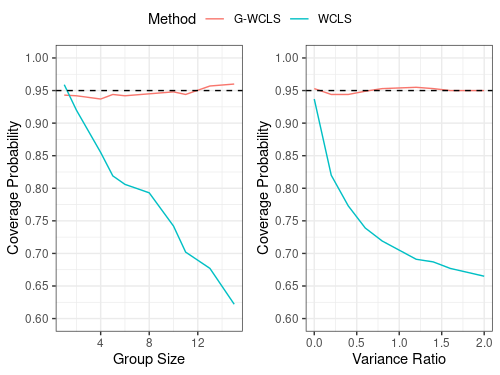
\includegraphics[scale=0.75]{Rplot.png}
% note that files may not be rotated
\caption{C-WCLS offers more valid $95\%$ confidence intervals than WCLS in Scenario II. Observed coverage probability varies by group size  ($G$) (total sample size fixed) ({\bf left}), and the variance of random intercept $b_g$ as a fraction of the variance of the random error term $e_g$ (\bf right).}
    \label{fig:undercoverage}
\end{figure}

\noindent {\bf Simulation Scenario III}.  In the third scenario, we assume the treatment effect for an individual depends on the average state of all individuals in the cluster. Therefore, we define the cluster-level moderator $\bar S_{t,g} = \frac{1}{G_g}\sum_{j=1}^{G_g} S_{t,j}$ and consider the generative model:
\begin{equation*}
Y_{t+1,j} = (-0.2 + b_g +  0.2 \cdot \bar S_{t,g}) \times (A_{t,j} -p_t(1|H_{t,j})) + 0.8 S_{t,j} + e_g + e_{t+1,j}
\end{equation*}
The proposed estimator again achieves the nominal 95\% coverage probability while the WCLS method does not (see Scenario III, Table~\ref{tab:simresults}).

\begin{table}[!th]
\centering
\begin{tabular}{c | ccccccc}
\hline
Scenario & Estimator & \# of Clusters & Cluster Size & Estimate & SE & RMSE & CP \\ \hline
\multirow{12}{*}{I} & C-WCLS & \multirow{2}{*}{25} & \multirow{2}{*}{10} & -0.198 & 0.035 & 0.036	 & 0.945 \\
& WCLS & & &  -0.200 & 0.036 & 0.035 & 0.956 \\  \cdashline{2-8}
& C-WCLS & \multirow{2}{*}{25} & \multirow{2}{*}{25} & -0.199 & 0.022 & 0.023 & 0.948 \\
& WCLS & & &  -0.199 & 0.023 & 0.022 & 0.958 \\ \cdashline{2-8}
& C-WCLS & \multirow{2}{*}{50} & \multirow{2}{*}{10} & -0.198 & 0.025 & 0.027 & 0.935 \\
& WCLS & & &  -0.198 & 0.026 & 0.026 & 0.944 \\ \cdashline{2-8}
& C-WCLS & \multirow{2}{*}{50} & \multirow{2}{*}{25} & -0.198 & 0.016 & 0.016 & 0.950 \\
& WCLS & & &  -0.198 & 0.016 & 0.017 & 0.937 \\ \cdashline{2-8}
& C-WCLS & \multirow{2}{*}{100} & \multirow{2}{*}{10} & -0.199 & 0.018 & 0.018 & 0.949 \\
& WCLS & & &  	-0.198& 0.018 & 0.019 & 0.949 \\ \cdashline{2-8}
& C-WCLS & \multirow{2}{*}{100} & \multirow{2}{*}{25} &  -0.198 & 0.011 & 0.012  & 0.941 \\
& WCLS & & &  -0.199 & 0.011 & 	0.012 & 0.944 \\ \hline
\multirow{12}{*}{II} & C-WCLS & \multirow{2}{*}{25} & \multirow{2}{*}{10} & -0.199 & 0.070 & 0.076 & 0.935 \\
& WCLS & & &  -0.201 & 0.041 & 0.076 & 0.710 \\  \cdashline{2-8}
& C-WCLS & \multirow{2}{*}{25} & \multirow{2}{*}{25} & -0.196 & 0.065 & 0.071 & 	0.933 \\
& WCLS & & &  -0.200 & 0.026 & 0.065 & 0.557 \\ \cdashline{2-8}
& C-WCLS & \multirow{2}{*}{50} & \multirow{2}{*}{10} & -0.200 & 0.051 & 0.049 & 0.957 \\
& WCLS & & &  -0.200 & 0.029 & 0.052 & 0.723 \\ \cdashline{2-8}
& C-WCLS & \multirow{2}{*}{50} & \multirow{2}{*}{25} & -0.200 & 0.047 & 0.049 & 0.947 \\
& WCLS & & &  -0.199 & 0.019 & 0.048 & 0.555 \\ \cdashline{2-8}
& C-WCLS & \multirow{2}{*}{100} & \multirow{2}{*}{10} & -0.198  & 0.036 & 0.035 & 0.955 \\
& WCLS & & &  -0.198 & 0.021 & 0.037 & 0.718 \\ \cdashline{2-8}
& C-WCLS & \multirow{2}{*}{100} & \multirow{2}{*}{25} & -0.198  & 0.033 & 0.035 & 0.942 \\
& WCLS & & &  -0.199 & 0.013 & 0.032 & 0.583 \\ \hline
\multirow{12}{*}{III} & C-WCLS & \multirow{2}{*}{25} & \multirow{2}{*}{10} & -0.199 & 0.070 & 0.073 & 0.948 \\
& WCLS & & &  -0.202 & 0.041 & 0.074 & 0.734 \\  \cdashline{2-8}
& C-WCLS & \multirow{2}{*}{25} & \multirow{2}{*}{25} & -0.196 & 0.066 & 0.069 & 0.931 \\
& WCLS & & &  -0.200 & 0.026 & 0.068 & 0.563 \\ \cdashline{2-8}
& C-WCLS & \multirow{2}{*}{50} & \multirow{2}{*}{10} & -0.198 & 0.051 & 0.052 & 0.941 \\
& WCLS & & &  -0.199 & 	0.029 & 0.052 & 0.742 \\ \cdashline{2-8}
& C-WCLS & \multirow{2}{*}{50} & \multirow{2}{*}{25} & -0.199 & 0.047 & 0.048 & 0.946 \\
& WCLS & & &  -0.200 & 0.018 & 0.048 & 0.561 \\ \cdashline{2-8}
& C-WCLS & \multirow{2}{*}{100} & \multirow{2}{*}{10} & -0.200 & 0.036 & 0.037 & 0.946 \\
& WCLS & & &  	-0.200 & 0.021 & 0.037 & 0.740 \\ \cdashline{2-8}
& C-WCLS & \multirow{2}{*}{100} & \multirow{2}{*}{25} & -0.201 & 0.034 & 0.033 & 0.956 \\
& WCLS & & &  -0.198 & 0.013 & 0.034 & 0.555 \\ \hline
\end{tabular}
\caption{Simulation: cluster-based weighted-centered least squares (C-WCLS) and weighted-least squares estimator (WCLS) comparison for Scenario I, II, and III.}
\label{tab:simresults}
\end{table}

% \hs{4. Demonstrate indirect effect}

\noindent {\bf Simulation Scenario IV}.  The fourth scenario considers the indirect effect.  For individual $j$ at decision point $t$, we construct the total effect as $TE_{t,j} = \sum_{j^\prime \neq j} \{A_{t,j^\prime} - \tilde p_{t, j^\prime} ( 1 \mid H_t) \} (\beta_{20} + \beta_{21} S_{t,j^\prime})$, where $\beta_{20} = -0.1$ and $\beta_{21} = 0.2$. The generative model is given by:
\begin{equation*}
    Y_{t+1,j} = (-0.2 + b_g +  0.2 \cdot \bar S_{t,g}) \times \{A_{t,j} -p_t(1|H_{t,j})\}+ 0.8 S_{t,j} +TE_{t,j} +e_g +e_{t+1,j}
\end{equation*}
This model implies a marginal indirect effect equal to $\beta_1^{(IE)} = \beta_{20} = -0.1$. Table~\ref{tab:simresults_indirect} presents the results.  We see that the proposed indirect estimator exhibited nearly no bias and achieved the nominal coverage probability.

\begin{table}[!th]
\centering
\begin{tabular}{c | cccccc}
\hline
Scenario & \# of Clusters & Cluster Size & Estimate & SD & RMSE & CP \\ \hline
\multirow{6}{*}{IV} & 25 & 10 & -0.097 & 0.028 & 0.029 & 0.958 \\
& 25 & 25 & -0.101 & 0.017 &  0.019 & 0.942 \\
& 50 & 10 & -0.097 & 0.020 & 0.021 & 0.953 \\
& 50 & 25 & -0.100 & 0.013 & 0.013 & 0.942 \\
& 100 & 10 & -0.097 & 0.015 & 0.015 & 0.943 \\
& 100 & 25 &  -0.100 & 0.009 & 0.009 & 0.944 \\ \hline
\end{tabular}
\caption{Simulation: C-WCLS for estimation of indirect effects.}
\label{tab:simresults_indirect}

\end{table}

\section{Case Study: Intern Health Study}
\label{section:casestudy}

The Intern Health Study (IHS) was a 6-month MRT on 1,565 medical interns where four types of weekly notification - mood, activity, sleep, or none -- were randomly assigned with equal probability to each subject~\cite{Necamp2020} (see Section~\ref{section:motex}).
In IHS,  273 institutions and 14 specialties were observed.   Here, we assess the effect of the three types of notifications (mood, activity, and sleep) compared to no notifications on the weekly average of self-reported mood scores and log step-count  for the population of interns.  See Appendix~\ref{app:IHSadditionalanalysis} for an additional analysis of log sleep minutes.  Due to high levels of missing data, weekly average mood scores and were computed from multiply imputed daily self-reported scores.  Similar imputation was performed for daily log step-counts and daily log sleep minutes. See~\cite{Necamp2020} for further details.

%\zw{isn't Likert five levels?} in pic from https://www.jmir.org/2020/3/e15033/pdf it shows 1-10.  Data also seems to be on that scale.
Let $t=1,\ldots,T$ denote the weekly decision points at which the individual is randomized to the various types of notifications.  Because of the form of the intervention, all participants were available for this intervention throughout the study; i.e., $I_t \equiv 1$. The proximal outcome~$Y_{j,t+1}$ is weekly mood score, which is reported on a Likert scale  taking values from 1 to 10 (higher scores mean better mood). We collapse notifications to a binary variable, i.e., $A_{t,j}=1$ if the individual was assigned to receive either mood, activity, or sleep notifications on week $t$; otherwise, $A_{t,j}= 0$ and no notifications were sent that week. At any occasion $t$, an individual's notification randomization probabilities were only dependent of their past observed history~$H_{t,j}$. For simplicity, we start with clusters beingare constructed based on medical specialty.  The average cluster size was 120; the first and third quartile were 56 and 140 respectively, with maximum and minimum sizes of 353 and 24.  For every individual in each cluster at each decision point we compute the average prior weekly mood score for all others in the cluster, denoted $\bar Y_{-j, t}$ for the $j$th individual in the cluster.  We consider two moderation analyses that can both be expressed as
$$
\beta(t; S_t) = \beta_0 + \beta_1 \cdot Y_{t-1,j} + \beta_2 \bar Y_{t-1,-j}.
$$

The first set of moderation analyses considers the standard moderation analysis where only individual-level moderators are included (i.e., $\beta_2 = 0$), with or without accounting for cluster-level moderation effect heterogeneity. Table~\ref{tab:IHS_direct} presents the results and compares our proposed approach against the WCLS approach from~\cite{Boruvkaetal}.  In this case, the effects do not change too much for the average weekly mood analysis; however, the significant effect of messages on weekly log step count under the traditional MRT analysis becomes insignificant when accounting for cluster effects.
% \zw{This is excellent. I suggest we move Table 5, extending the present Table 4. This shows C-WCLS may produce different inferential results, which in the presence of clusters, can be more trustworthy than a classical WCLS.}

The second moderation analysis lets $\beta_2$ be a free parameter, enabling novel moderation analyses that accounts for the average weekly previous mood score of other individuals.  Table~\ref{tab:IHS_direct} presents the results.  Here, we see that the constant term~$\beta_0$ becomes negative but insignificant while the new term $\beta_2$ is positive and significant.  The results suggest the average mood of others in the cluster may moderate the effect of notifications.  Therefore, the impact of a notification is larger when the average mood score of others in the specialty is large while the individual's score is low.   Similar results hold for the log step-count analysis.
% \zw{This reminds me of a separate line of work that parallels that of model diagnostics/selection in MSM or SNMM. But you may argue that this is all about projection, in which case it perhaps warrants brief discussion, e.g., in the discussion. }  I agree that it's important issue but for this paper I would argue that it's more about the projection interpretation :)

\begin{table}[!th]
\centering
\begin{tabular}{c |c | crrrr}
\hline
Outcome & Setting & Variables & Estimate & Std. Error & t-value & p-value \\ \hline
\multirow{7}{*}{Mood} & \multirow{2}{*}{WCLS} & $\beta_0$ & 0.369 & 0.086 & 4.268 & 0.000 \\
& & $\beta_1$ & -0.055 & 0.011 & -4.822 & 0.000 \\ \cline{2-7}
& \multirow{2}{*}{C-WCLS} & $\beta_0$ & 0.350 & 0.103 & 3.401 & 0.001 \\
& & $\beta_1$ & -0.053 & 0.014 & -3.868 & 0.000 \\ \cline{2-7}
& \multirow{3}{*}{C-WCLS} & $\beta_0$ & -0.238 & 0.282 & -0.842 & 0.401 \\
& & $\beta_1$ & -0.054 & 0.014 & -3.973 & 0.000 \\
& & $\beta_2$ & 0.083 & 0.037 & 2.241 & 0.026 \\ \hline
\multirow{7}{*}{Steps} & \multirow{2}{*}{WCLS} & $\beta_0$ & 0.729 & 0.295 & 2.472 & 0.015 \\
& & $\beta_1$ & -0.037 & 0.015 & -2.484 & 0.015 \\ \cline{2-7}
& \multirow{2}{*}{C-WCLS} & $\beta_0$ & 0.622 & 0.384 & 1.618 & 0.108 \\
& & $\beta_1$ & -0.031 & 0.019 & -1.580 & 0.117 \\ \cline{2-7}
& \multirow{3}{*}{C-WCLS} & $\beta_0$ & -2.095 & 1.248 & -1.678 & 0.094 \\
& & $\beta_1$ & -0.034 & 0.019 & -1.745 & 0.083 \\
& & $\beta_2$ & 0.143 & 0.062 &2.330 & 0.020 \\ \hline
\end{tabular}
\caption{Moderation analysis for the effect of notifications on average weekly mood scores and log step counts respectively in IHS. WCLS estimates use the estimator in~\cite{Boruvkaetal}, while the C-WCLS estimates use our proposed estimator.}
\label{tab:IHS_direct}
\end{table}

Finally, we consider indirect moderation effect analyses.   In this analysis, clusters are constructed based on medical specialty and institution.  This was done as interference was only likely when interns are in close geographic proximity.   Here, we consider the marginal indirect effect (e.g., no moderators) both when the individual did not receive the intervention and when the individual did receive an intervention at decision time~$t$.  Table~\ref{tab:IHS_indirect} presents the results.  In this case, the estimated indirect effects are weaker than the direct effects by a factor of approximately 10.  Even a weak effect may be unexpected as none of the content in the push notifications was aimed at impacting other individuals' behavior. The fact that there is any signal for the impact on proximal mood implies the scientific team may wish to consider interventions that target these indirect effects more explicitly, either in the framing of the messages or in messaged aimed at impacting the overall group. For the other proximal outcomes, we see limited evidence of an indirect effect.  This implies that the scientific team, when building an optimal JITAI for these behaviors, may decide to ignore the indirect effects and instead solely focus on its impact on the individual who receives this push notification.

\begin{table}[!th]
\centering
\begin{tabular}{c | crrrr}
\hline
Outcome & Variables & Estimate & Std. Error & t-value & p-value \\ \hline
\multirow{2}{*}{Mood} & $\tilde \beta_0$ & 0.015 & 0.017 & 0.901 & 0.184 \\
& $\tilde \beta_1$ & 0.027 & 0.019 & 1.411 & 0.079 \\ \hline
\multirow{2}{*}{Steps} & $\tilde \beta_0$ & 0.023 & 0.051 & 0.454 & 0.325\\
& $\tilde \beta_1$ & 0.052 & 0.060 & 0.871 & 0.192 \\ \hline
\multirow{2}{*}{Sleep} & $\tilde \beta_0$ & 0.034 & 0.035 & 0.980 & 0.164\\
& $\tilde \beta_1$ & 0.034 & 0.035 & 0.980 & 0.164\\ \hline
\end{tabular}
\caption{Moderation analysis for the indirect effect of notifications on average weekly mood scores, log step counts, and log sleep minutes respectively in IHS.  Coefficient $\tilde \beta_0$ represents the indirect effect under $A_{j,t} = 0$, while the coefficient $\tilde \beta_1$ represents the indirect effect under $A_{j,t} = 1$.}
\label{tab:IHS_indirect}
\end{table}

\section{Discussion}

Here we consider the causal excursion effect in the presence of a priori known clusters.  We have extended the causal excursion effect to naturally account for cluster information. In particular, both direct and indirect excursion effects have been formalized in the context of MRT to account for potential interference.  The effects described in this paper are most important when using MRT data to build optimized JITAIs for deployment in an mHealth package. Specifically, the estimation procedure for the direct excursion effect accounts for within-cluster correlation in the proximal outcomes which helps the scientific team avoid making erroneous conclusions about intervention effectiveness using standard MRT methods.  Moreover, estimation of indirect effects allows the scientific team to answer questions about impact of interventions on other members of the same cluster.  Use of these methods provides empirical evidence for the scientific team to include or exclude intervention components that may have had unanticipated second order effects, or potentially lead to novel ways to improve the intervention component by revising the intervention to more explicitly account for cluster-level interference.  While this work represents a major step forward in the analysis of micro-randomized trial data, further work is required.  Specifically, extensions to be considered future work include accounting for overlapping communities and/or network (rather than cluster-only) structure~\citep{Ogburn2014,Mealli2019}, accounting for general non-continuous proximal outcomes such as binary or count outcomes~\citep{Qian2021}, penalization of the working model to allow for high-dimensional moderators, and a method to use the proposed approach to form warm-start policies at the individual level while accounting for group level information~\citep{Luckett2020}.


\section*{Acknowledgments}
The authors would like to thank the Intern Health Study (IHS) team at University of Michigan for substantive discussions, Professor Srijan Sen (Principal Investigator) for generously providing access to the IHS data, and the study participants of IHS for providing the data.  The draft also benefited from helpful comments from Professors Inbal Nahum-Shani and Peng Ding.


\bibliography{groupmrts}

\newpage

% \appendix

% \section{Technical Details}
% \label{app:techdetails}

% \begin{proof}{Proof of Lemma \ref{lemma:cond_effect}}
% We establish Lemma~\ref{lemma:cond_effect} for the direct effect~\eqref{eq:directavglineareffect}. For~$a_s \in \{ 0,1\}^{G}$, we consider
% \begin{align*}
% \E &\left[\left(\prod_{s=1}^{t-1} p_s(a_s|H_s(\bar a_{s-1})) \right) \left( \prod_{j^\prime \neq j} p_t(a_{t,j^\prime} \mid H_t(\bar a_{t-1})\right)
%  Y_{t+1,j} (\bar{a}_{t,-j}, (\bar a_{t-1,J},a)) {\bf 1}_{S_t(\bar a_t) = s} \right] \\
%  \E &\left[\left(\prod_{s=1}^{t-1} p_s(a_s|H_s(\bar a_{s-1})) \right) \left( \prod_{j^\prime \neq j} p_t(a_{t,j^\prime} \mid H_t(\bar a_{t-1}) \right) {\bf 1}_{S_t(\bar a_t) = s}  \E \left[ Y_{t+1,j} (\bar{a}_{t,-j}, (\bar a_{t-1,j},a)) \mid H_t (\bar a_{t-1}) \right] \right]
% \end{align*}
% since the history $H_t$ includes the moderator variable $S_t$ at time $t$. By consistency,~$H_t(\bar{A}_{t-1}) = H_t$ so the above is equal to
%  \begin{equation} \label{eq:cons_version}
% \E \left[\left(\prod_{s=1}^{t-1} p_s(a_s|H_s) \right) \left( \prod_{j^\prime \neq J} p_t(a_{t,j^\prime} \mid H_t \right)  {\bf 1}_{S_t(\bar a_t) = s}
%  \E \left[ Y_{t+1,j} (\bar{a}_{t,-j}, (\bar a_{t-1,j},a))   \given H_t \right]  \right]
%  \end{equation}
% Sequential ignorability implies that
% \begin{align*}
%  \E &\left[ Y_{t+1,j} (\bar{a}_{t,-j}, (\bar a_{t-1,j},a)) \given H_t \right]  \\
%  = \E &\left[ Y_{t+1,j} (\bar{a}_{t,-j}, (\bar a_{t-1,j},a)) \given H_{t}, A_{t,j} = a \right]
% \end{align*}
% Summing over all potential outcomes and normalizing yields
% \begin{align*}
% \E &\left[ \sum_{\bar{a}_{t-1}} \frac{\left(\prod_{s=1}^{t-1} p_s(a_s|H_s) \right) \left( \prod_{j^\prime \neq j} p_t(a_{t,j^\prime} \mid H_t \right)  {\bf 1}_{S_t(\bar a_t) = s}}{\E [ \left(\prod_{s=1}^{t-1} p_s(a_s|H_s) \right) \left( \prod_{j^\prime \neq j} p_t(a_{t,j^\prime} \mid H_t \right)  {\bf 1}_{S_t(\bar a_t) = s}]}
%  \E \left[ Y_{t+1,j} (\bar{a}_{t,-j}, (\bar a_{t-1},a)) \given H_t, A_{t,j} = a \right] \, \right] \\
%  = \E &\left[ \sum_{\bar{a}_{t-1}} \frac{\left(\prod_{s=1}^{t-1} p_s(a_s|H_s) \right) \left( \prod_{j^\prime \neq j} p_t(a_{t,j^\prime} \mid H_t \right)  {\bf 1}_{S_t(\bar a_t) = s}}{\E [ \left(\prod_{s=1}^{t-1} p_s(a_s|H_s) \right) \left( \prod_{j^\prime \neq j} p_t(a_{t,j^\prime} \mid H_t \right)  {\bf 1}_{S_t(\bar a_t) = s}]}
%   \E \left[ Y_{t+1,j} (\bar{a}_{t,-j}, (\bar a_{t-1},a)) \given H_t, A_t = a \right] \given S_t = s \right] \\
%   = \E &\left[ \E \left[ Y_{t+1,j}  \given H_t, A_t = a \right] \given S_t = s \right].
% \end{align*}
% In the final equation, the outer expectation is with respect to the history~$H_t$ conditional on~$S_t=s$.  That is, over \emph{both} past treatments~$A_s$
% and past observations~$O_s$ for $s < t$ as well as over current treatments for $A_{t,j^\prime}$ for $j^\prime \neq j$. The above shows
% $$
% \E \left[ Y_{t+1} (\bar{A}_{t,-j}, (\bar A_{t-1,j},a)) \mid S_t (\bar a_t) = s \right] = \E \left[ \E \left[Y_{t+1, j}  \given H_t, A_{t,j} = a \right] \given S_t = s \right].
% $$
% Averaging over individuals in the group $j \in [G]$ group size completes the proof.
% The proof for the indirect effect follows the exact same structure.
% \end{proof}

% \subsection{Lemma~\ref{lemma:asymnorm}}
% \label{app:asymptotics}

% We next provide a detailed proof of asymptotic normality and consistency
% for the weighted-centered least squares estimator.

% \begin{proof}[Proof of consistency for direct and indirect effects]
% The solutions~$(\hat \alpha,\hat \beta)$ that minimize equation~\eqref{eq:directwcls} are consistent estimators for the
% solutions that minimize the following
% \[
% \E \left[ \frac{1}{G} \sum_{j=1}^G \sum_{t=1}^T W_{t,j} \left( Y_{t+1,j} - g_t(H_t)^\prime \alpha
% -  (A_{t,j} - \tilde{p}_t (1 \given S_t) ) f_t (S_t)^\prime \beta \right)^2 \right]
% \]
% Differentiating the above equation with respect to~$\alpha$
% yields a set of~$p$ estimating equations.
% \begin{align*}
% 0_{q^\prime}&= \E \left[ \frac{1}{G} \sum_{j=1}^G \sum_{t=1}^T W_{t,j} \left( Y_{t+1,j} - g_t(H_t)^\prime \alpha -  (A_{t,j} - \tilde{p}_t (1 \given S_t) ) f_t (S_t)^\prime \beta \right) g_t(H_t) \right]
% \end{align*}
% We note that
% $$
% \E \left[ W_{t,J} (A_{t,J} - \tilde{p}_t (1 \given S_t) )
% f_t (S_t)^\prime \beta \given H_t \right] = 0.
% $$
% Therefore, we have,
% \begin{align*}
% 0_{p}&= \E \left[ \frac{1}{G} \sum_{j=1}^G \sum_{t=1}^T (g_t(H_t) \E \left[ W_{t,j} Y_{t+1, j} \right] - g_t(H_t)  g_t(H_t)^\prime \alpha) \right] \\
% \Rightarrow \alpha  &= \E \left[ \frac{1}{G} \sum_{j=1}^G \sum_{t=1}^T g_t(H_t)  g_t(H_t)^\prime  \right]^{-1} E \left[ \frac{1}{G} \sum_{j=1}^G \sum_{t=1}^T g_t(H_t) \E \left[ W_{t,j} Y_{t+1, j} \right] \right]
% \end{align*}
% We note that
% \begin{align*}
% &\E \left[ W_{t,J} (A_{t,J} - \tilde{p}_t (1 \given S_t) )
% g_t (H_t)^\prime \alpha \right] = 0, \quad \text{and} \\
% &\E \left[ W_{t,J} (A_{t,J} - \tilde{p}_t (1 \given S_t) )
% Y_{t+1,J} \right] =
% \tilde{p}_t (1 \given S_t) (1- \tilde{p}_t (1 \given S_t)) \beta (t; S_t)
% \end{align*}
% Now differentiating with respect to~$\beta$ yields
% \begin{align*}
% 0_{q}&= \E \left[ \sum_{t=1}^T W_{t,J} \left( Y_{t+1,J} - g_t(H_t)^\prime \alpha
% -  (A_{t,J} - \tilde{p}_t (1 \given S_t) ) f_t (S_t)^\prime \beta \right) (A_{t,J} - \tilde{p}_t(1 \given S_t)) f_t (S_t) \right] \\
% 0_{q}&= \E \left[ \sum_{t=1}^T \tilde{p}_t (1 \given S_t) (1- \tilde{p}_t (1 \given S_t)) \left( \beta (t; S_t) - f_t (S_t)^\prime \beta^\star \right) f_t (S_t) \right]
% \end{align*}
% Then we have
% \begin{align*}
% \beta^\star &= \E\left[ \sum_{t=1}^T  \tilde{p}_t (1 \given S_t) (1- \tilde{p}_t (1 \given S_t)) f_t(S_t) f_t(S_t)^\prime \right]^{-1} \E\left[ \sum_{t=1}^T  \tilde{p}_t (1 \given S_t) (1- \tilde{p}_t (1 \given S_t)) f_t(S_t) \beta (t;S_t) \right]
% \end{align*}
% Under assumption~\ref{ass:directeffect}, we have that $\beta = \beta^\star$ which guarantees consistency.

% We next consider the indirect effect estimator.  Recall that
% $$
% \tilde{p}^\star_t (1 \given S_t) = \frac{\tilde{p}_t (0,1 \given S_t)}{\tilde{p}_t (0,0 \given S_t)+\tilde{p}_t (0,1 \given S_t)}
% $$
% is the replacement for $\tilde p(1 \mid S_t)$ in the direct effect for centering.  If we make the assumption that $\tilde p_t (0,1 \mid S_t) = \tilde p_t (0 \mid S_t) \tilde p_t (1 \mid S_t)$ then $\tilde{p}^\star_t (1 \given S_t) = \tilde{p}_t (1 \given S_t)$; however, we provide the proof in complete generality. The estimates that minimize equation~\eqref{eq:indirectwcls} are consistent estimators for the solutions that minimize the following
% \[
% \E \left[ \sum_{t=1}^T W_{t,J, J^\prime} \left( Y_{t+1,J} - g_t(H_t)^\prime \alpha
% -  (1-A_{t,J}) (A_{t,J^\prime} - \tilde{p}^\star_t (1 \given S_t) ) f_t (S_t)^\prime \beta \right)^2 \right]
% \]
% Differentiating the above equation with respect to~$\alpha$
% yields a set of~$p$ estimating equations.
% \begin{align*}
% 0_{p}&= \E \left[ \sum_{t=1}^T W_{t,J,J^\prime} \left( Y_{t+1,J} - g_t(H_t)^\prime \alpha
% -  (1-A_{t,J}) (A_{t,J^\prime} - \tilde{p}_t^\star (1 \given S_t) ) f_t (S_t)^\prime \beta \right) g_t(H_t) \right]
% \end{align*}
% We note that
% $$
% \E \left[ W_{t,J, J^\prime} (1-A_{t,J}) (A_{t,J^\prime} - \tilde{p}_t^\star (1 \given S_t) )
% f_t (S_t)^\prime \beta \given H_t \right] = 0.
% $$
% Therefore, we have,
% \begin{align*}
% 0_{p}&= \E \left[ \sum_{t=1}^T (g_t(H_t) \E \left[ W_{t,J,J^\prime} Y_{t+1, J} \right] - g_t(H_t)  g_t(H_t)^\prime \alpha) \right] \\
% \Rightarrow \alpha  &= \E \left[ \frac{1}{G} \sum_{j=1}^G \sum_{t=1}^T g_t(H_t)  g_t(H_t)^\prime  \right]^{-1} E \left[ \sum_{t=1}^T g_t(H_t) \E \left[ W_{t,J, J^\prime} Y_{t+1, J} \right] \right]
% \end{align*}
% First, we show that
% \begin{align*}
% &\E \left[ W_{t,J, J^\prime} (1-A_{t,J}) (A_{t,J^\prime} - \tilde{p}_t^\star (1 \given S_t) )
% \mid H_t \right] \\
% = &\sum_{a^\prime \in \{0,1\}} \E \left[ \tilde{p}_t (0,a^\prime \mid S_t)  (a^\prime - \tilde{p}_t^\star (1 \given S_t) )
% \mid H_t, A_t = 0, A_{t,J^\prime} = a^\prime \right]\\
% =& \tilde{p}_t (0,1 \mid S_t)  (1 - \frac{\tilde{p}_t (0,1 \given S_t)}{\tilde{p}_t (0,0 \given S_t)+\tilde{p}_t (0,1 \given S_t)} ) -  \tilde{p}_t (0,0 \mid S_t) \frac{\tilde{p}_t (0,1 \given S_t)}{\tilde{p}_t (0,0 \given S_t)+\tilde{p}_t (0,1 \given S_t)} = 0
% \end{align*}
% and
% \begin{align*}
% &\E \left[ W_{t,J, J^\prime} (1-A_{t,J}) (A_{t,J^\prime} - \tilde{p}_t^\star (1 \given S_t) )^2
% \mid H_t \right] \\
% =& \tilde{p}_t (0,1 \mid S_t) \left( \frac{\tilde{p}_t (0,0 \given S_t)}{\tilde{p}_t (0,0 \given S_t) +\tilde{p}_t (0,1 \given S_t)} \right)^2 + \tilde{p}_t (0,0 \mid S_t) \left( \frac{\tilde{p}_t (0,1 \given S_t)}{\tilde{p}_t (0,0 \given S_t)+\tilde{p}_t (0,1 \given S_t)} \right)^2 \\
% =& ( \tilde{p}_t (0,0 \mid S_t) + \tilde{p}_t (0,1 \mid S_t) ) \tilde{p}_t^\star (1 \mid S_t) (1- \tilde{p}_t^\star (1 \mid S_t)).
% \end{align*}
% This implies that
% \begin{align*}
% &\E \left[ W_{t,J, J^\prime} (1-A_{t,J}) (A_{t,J^\prime} - \tilde{p}_t^\star (1 \given S_t) )
% g_t (H_t)^\prime \alpha \right] = 0, \quad \text{and} \\
% &\frac{\E \left[ W_{t,J, J^\prime} (1-A_{t,J}) (A_{t,J^\prime} - \tilde{p}_t^\star (1 \given S_t) )
% Y_{t+1,J} \right]}{\tilde{p}_t (0,0 \mid S_t) + \tilde{p}_t (0,1 \mid S_t)} = \tilde{p}_t^\star (1 \mid S_t) (1- \tilde{p}_t^\star (1 \mid S_t)) \beta^{(IE)} (t; S_t).
% \end{align*}
% Now differentiating with respect to~$\beta$ yields
% \begin{align*}
% 0_{q}&= \E \left[ \sum_{t=1}^T ( \tilde{p}_t (0,0 \mid S_t) + \tilde{p}_t (0,1 \mid S_t) ) \tilde{p}_t^\star (1 \mid S_t) (1- \tilde{p}_t^\star (1 \mid S_t)) \left( \beta^{(IE)} (t; S_t) - f_t (S_t)^\prime \beta^{\star \star} \right) f_t (S_t) \right]
% \end{align*}
% Under assumption~\ref{ass:indirecteffect}, we have that $\beta = \beta^{\star \star}$ which guarantees consistency.
% \end{proof}

% \begin{proof}[Proof of Asymptotic Normality]
% We now consider the issue of asymptotic normality.  First, let
% \[
% \epsilon_{t,j} = Y_{t+1,j} - g_t(H_t)^{\prime} \alpha^\star - (A_{t,j}-\tilde{p}_t(1 \mid S_t)) f_t(S_t)^{\prime} \beta^\star,
% \]
% $\hat{\theta} = (\hat{\alpha}, \hat{\beta})$, and $\theta^\star = (\alpha^\star, \beta^\star)$.
% Since $S_t \subset H_t$ define $h_{t,j}(H_t)^\prime = (g_t(H_t)^\prime, (A_{t,j}-\tilde{p}_t(1 \given S_t)) f_t(S_t)^\prime)$. Then
% \begin{align*}
% \sqrt{M} ( \hat{\theta} - \theta^\star )
%   &= \sqrt{M} \bigg \{ \mathbb{P}_M \bigg( \frac{1}{G_m} \sum_{j=1}^{G_m} \sum_{t=1}^T W_{t,j} h_{t,j}(H_t) h_{t,j}(H_t)^\prime \bigg)^{-1} \bigg[
%     \mathbb{P}_M \bigg( \frac{1}{G_m} \sum_{j=1}^{G_m} \sum_{t=1}^T W_{t,j}
%     Y_{t+1,j} h_{t,j}(H_t) \bigg) \\
%   &- \mathbb{P}_M \bigg( \frac{1}{G_m} \sum_{j=1}^{G_m}
%   \sum_{t=1}^T W_{t,j} h_{t,j}(H_t) h_{t,j}(H_t)^\prime \bigg)
%     \theta^\star \bigg] \bigg \} \\
%   &= \sqrt{M} \bigg \{ E \bigg[
%   \frac{1}{G} \sum_{j=1}^G \sum_{t=1}^T W_{t,j} h_{t,j}(H_t)
%   h_{t,j}(H_t)^\prime \bigg]^{-1} \\
%   &\bigg[ \mathbb{P}_M \bigg( \frac{1}{G_m} \sum_{j=1}^{G_m} \sum_{t=1}^T
%     W_{t,j} \epsilon_{t,j} h_{t,j}(H_t) \bigg) \bigg] \bigg \} + o_p ( {\bf 1} )
% \end{align*}
% By definitions of $\alpha^\star$ and $\beta^\star$ and the previous consistency argument
% \[
% E \bigg[
%   \frac{1}{G} \sum_{j=1}^G \sum_{t=1}^T W_{t,j} h_{t,j}(H_t)
%   h_{t,j}(H_t)^\prime \bigg]  = 0
% \]
% Then under moments conditions, we have asymptotic normality with variance $\Sigma_{\theta}$ given by
% \begin{align*}
% \Sigma_{\theta} &= E \left[ \frac{1}{G} \sum_{j=1}^G \sum_{t=1}^T W_{t,j} h_{t,j}(H_t) h_{t,j}(H_t)^\prime \right]^{-1} \\
%                 &E \left[ \frac{1}{G} \sum_{j=1}^G \sum_{t=1}^T W_{t,j} \epsilon_{t,j} h_{t,j}(H_t)
%                   \times  \frac{1}{G} \sum_{j=1}^G \sum_{t=1}^T W_{t,j} \epsilon_{t,j} h_{t,j}(H_t)^\prime \right] \\
%                 &E \left[ \frac{1}{G} \sum_{j=1}^G \sum_{t=1}^T W_{t,j} h_{t,j}(H_t) h_{t,j}(H_t)^\prime \right]^{-1}
% \end{align*}
% Due to centering, the expectation of the matrix
% $W_{t,J} h_{t,J}(H_t) h_{t,J} (H_t)^\prime$ is block diagonal and
% the sub-covariance matrix~$\Sigma_{\beta}$ can be extracted and is equal to
% \begin{align*}
%  \Sigma_{\beta} &=  \left[ \sum_{t=1}^T E[ (A_{t,J} - \tilde{p}_t (1 \mid S_t)
%                   )^2 W_{t,J} f_t (S_t) f_t (S_t)^\prime ] \right]^{-1} \\
%   &\cdot E \bigg[ \sum_{t=1}^T W_{t,J} \epsilon_{t,J}
%                   (A_{t,J} - \tilde{p}_t( 1 \mid S_t)) f_t(S_t)
%           \times  \sum_{t=1}^T W_{t,J} \epsilon_{t,J}
%                   (A_{t,J} - \tilde{p}_t( 1 \mid S_t)) f_t(S_t)^\prime
%                   \bigg] \\
%  &\, \cdot \left[ \sum_{t=1}^T E[ (A_{t,J} - \tilde{p}_t (1 \mid S_t)
%                   )^2 W_{t,J} f_t (S_t) f_t (S_t)^\prime ] \right]^{-1}
% \end{align*}
% as desired.

% We next consider asymptotic normality in the indirect setting.  First, let
% \[
% \epsilon_{t,j,j^\prime} = Y_{t+1,j} - g_t(H_t)^{\prime} \alpha^{\star \star} - (1 - A_{t,j})(A_{t,j^\prime}-\tilde{p}^\star_t(1 \mid S_t)) f_t(S_t)^{\prime} \beta^{\star \star},
% \]
% $\hat{\theta} = (\hat{\alpha}, \hat{\beta})$, and $\theta^\star = (\alpha^{\star \star}, \beta^{\star \star})$.
% Since $S_t \subset H_t$ define $h_{t,j,j^\prime}(H_t)^\prime = (g_t(H_t)^\prime, (1-A_{t,j}) (A_{t,j^\prime}-\tilde{p}^\star_t(1 \given S_t)) f_t(S_t)^\prime)$. Then $\sqrt{M} ( \hat{\theta} - \theta^{\star \star} )$ equals
% \begin{align*}
%   &\sqrt{M} \bigg \{ \mathbb{P}_M \bigg( \frac{1}{G_m \cdot (G_m-1)} \sum_{j=1}^{G_m} \sum_{j^\prime \neq j} \sum_{t=1}^T W_{t,j,j^\prime} h_{t,j,j^\prime}(H_t) h_{t,j,j^\prime}(H_t)^\prime \bigg)^{-1} \\
%   &\bigg[
%     \mathbb{P}_M \bigg( \frac{1}{G_m \cdot (G_m - 1)} \sum_{j=1}^{G_m} \sum_{j^\prime \neq j} \sum_{t=1}^T W_{t,j} Y_{t+1,j} h_{t,j,j^\prime}(H_t) \bigg)  \\
%   &- \mathbb{P}_M \bigg( \frac{1}{G_m \cdot (G_m - 1)} \sum_{j=1}^{G_m}\sum_{j^\prime \neq j}
%   \sum_{t=1}^T W_{t,j,j^\prime} h_{t,j, j^\prime}(H_t) h_{t,j, j^\prime}(H_t)^\prime \bigg)
%     \theta^\star \bigg] \bigg \} \\
%   = &\sqrt{M} \bigg \{ E \bigg[
%   \frac{1}{G (G-1)} \sum_{j=1}^G \sum_{j^\prime \neq j} \sum_{t=1}^T W_{t,j,j^\prime} h_{t,j, j^\prime}(H_t) h_{t,j, j^\prime}(H_t)^\prime \bigg]^{-1} \\
%   &\bigg[ \mathbb{P}_M \bigg( \frac{1}{G_m \cdot (G_m-1)} \sum_{j=1}^{G_m} \sum_{j^\prime \neq j} \sum_{t=1}^T W_{t,j,j^\prime} \epsilon_{t,j, j^\prime} h_{t,j,j^\prime}(H_t) \bigg) \bigg] \bigg \} + o_p ( {\bf 1} )
% \end{align*}
% By definitions of $\alpha^{\star \star}$ and $\beta^{\star \star}$  and the previous consistency argument
% \[
% E \bigg[
%   \frac{1}{G \cdot (G-1)} \sum_{j=1}^G \sum_{j^\prime \neq j} \sum_{t=1}^T W_{t,j,j^\prime} h_{t,j,j^\prime}(H_t)
%   h_{t,j,j^\prime}(H_t)^\prime \bigg]  = 0
% \]
% Then under moments conditions, we have asymptotic normality with variance $\Sigma_{\theta}$ given by
% \begin{align*}
% \Sigma_{\theta} &= E \left[ \frac{1}{G \cdot (G-1)} \sum_{j=1}^G \sum_{j^\prime \neq j} \sum_{t=1}^T W_{t,j,j^\prime} h_{t,j,j^\prime}(H_t) h_{t,j,j^\prime}(H_t)^\prime \right]^{-1} \\
%                 &E \left[ \frac{1}{G (G-1)} \sum_{j=1}^G \sum_{j^\prime \neq j} \sum_{t=1}^T W_{t,j, j^\prime} \epsilon_{t,j, j^\prime} h_{t,j, j^\prime}(H_t)
%                   \times  \frac{1}{G(G-1)} \sum_{j=1}^G \sum_{j^\prime \neq j} \sum_{t=1}^T W_{t,j} \epsilon_{t,j, j^\prime} h_{t,j, j^\prime}(H_t)^\prime \right] \\
%                 &E \left[ \frac{1}{G \cdot (G-1)} \sum_{j=1}^G \sum_{j^\prime \neq j} \sum_{t=1}^T W_{t,j,j^\prime} h_{t,j,j^\prime}(H_t)
%   h_{t,j,j^\prime}(H_t)^\prime  \right]^{-1}
% \end{align*}
% Due to centering, the expectation of the matrix
% $W_{t,J, J^\prime} h_{t,J,J^\prime}(H_t) h_{t,J, J^\prime} (H_t)^\prime$ is block diagonal and
% the sub-covariance matrix~$\Sigma_{\beta}$ can be extracted and is equal to
% \begin{align*}
%  \Sigma_{\beta} &=  \left[ \sum_{t=1}^T E[ (1- A_{t,J}) (A_{t,J^\prime} - \tilde{p}_t^\star (1 \mid S_t)
%                   )^2 W_{t,J, J^\prime} f_t (S_t) f_t (S_t)^\prime ] \right]^{-1} \\
%   &\cdot E \bigg[ \sum_{t=1}^T W_{t,J, J^\prime} \epsilon_{t,J, J^\prime}
%                   (1-A_{t,J}) (A_{t,J^\prime} - \tilde{p}_t( 1 \mid S_t)) f_t(S_t) \\
%           &\times  \sum_{t=1}^T W_{t,\tilde  J, \tilde J^\prime} \epsilon_{t, \tilde J, \tilde J^\prime}
%                   (1-A_{t,\tilde J}) (A_{t,\tilde J^\prime} - \tilde{p}_t^\star( 1 \mid S_t)) f_t(S_t)^\prime
%                   \bigg] \\
%  &\, \cdot \left[ \sum_{t=1}^T E[ (1-A_{t,J}) (A_{t,J^\prime} - \tilde{p}_t (1 \mid S_t)
%                   )^2 W_{t,J,J^\prime} f_t (S_t) f_t (S_t)^\prime ] \right]^{-1}
% \end{align*}
% as desired.
% \end{proof}

% % \section{Additional simulation details}
% % \label{app:simdetails}

% % Different scenarios were devised by setting $\beta_{11}^*$ to one of 0.2, 0.5, 0.8, giving respectively a small, medium, or large degree of moderation by $S_t$. Since $\eta_1$ and $\eta_2$ are nonzero, the treatment $A_t$ is assigned with a probability depending on both $S_t$ and past treatment $A_{t-1}$, for each $t$.

% % In the weighted and centered analysis, we parameterize and estimate $\tilde{p}_t$. In particular, $\tilde{p}_t(a;\hat{p}) = \hat{p}^a(1-\hat{p})^{1-a}$ where $\hat{p} = \P_n \sum_{t=1}^T A_t/T$. The weights are set to $W_t = \hat{p}^{A_t}(1-\hat{p})^{1-A_t}/p_t(A_t|H_t)$ and the working model for $\E \left[W_tY_{t+1}|H_t \right]$ is $a_{10}+a_{11}S_t$ (i.e., $g_t(H_t)= (1, S_t)^T$). Thus the estimating function is given by: \hs{Is this necessary?}
% % % $$
% % %     \sum_{t=1}^T (Y_{t+1} - (a_{10}+a_{11}S_t) - (A_t - \hat{p})\beta_1)W_t
% % %     \left( \begin{array}{c}
% % %          (1,S_t)^T \\
% % %          A_t -\hat{p}
% % %     \end{array}  \right) =0
% % % $$


% % \hs{2.  Show under-coverage when $b_g$ interacts with centered treatments - provide intuition; Show under different group size the difference in estimation}

% % Unlike the above scenarios, the definition of indirect effect here excludes the observations with $A_{t,j} = 1$. Hence, we can make references on how interactions will influence the response $Y_{t+1,j}$ when treatment is absent. Weights are set to be $w'_{t,j,j'} = w_{t,j} \times w_{t,j'}$, and the corresponding estimation function is:
% % \begin{align*}
% %      \frac{1}{M} \sum_{m=1}^{M}  \binom{G_m}{2}^{-1}\sum_{j=1}^{G_m} \sum_{t=1}^T (&Y_{t+1,j} - (a_{10}+a_{11}S_{t,j}) - (1-A_{t,j}) \times \sum_{j^\prime \neq j} (A_{t,j^\prime} - \tilde p_{t, j^\prime} ( 1 \mid H_t) )\beta_2) \\
% %      &W'_t \left( \begin{array}{cc}
% %          (1,\bar S_{t,g})^T\\
% %          (1-A_{t,j}) \times \sum_{j^\prime \neq j} (A_{t,j^\prime} - \tilde p_{t, j^\prime} ( 1 \mid H_t) )
% %     \end{array}  \right) =0
% % \end{align*}

% \section{Proof of Lemma~\ref{lemma:samesies}}
% \label{app:samesies}

% \begin{proof}
% Consider the $W$-matrix for the direct effect asymptotic variance,
% \begin{align*}
%  &\frac{1}{G^2} \sum_{t, t^\prime} \sum_{j, j^\prime} \mathbb{E} \bigg[
%  W_{t,j} \epsilon_{t,j} (A_{t,j} - \tilde{p}_t( 1 \mid S_t))
%  W_{t^\prime,j^\prime} \epsilon_{t^\prime,j^\prime} (A_{t^\prime,j^\prime} - \tilde{p}_t( 1 \mid S_{t^\prime}))
%  f_t(S_t) f_{t^\prime}(S_{t^\prime})^\prime
%                   \bigg] \\
% =&\frac{1}{G^2} \sum_{t, t^\prime}\sum_{j, j^\prime} \mathbb{E} \bigg[
%  W_{t,j} \epsilon_{t,j} (A_{t,J} - \tilde{p}_t( 1 \mid S_t))
%  W_{t^\prime,j^\prime} \epsilon_{t^\prime,j^\prime} (A_{t^\prime,j^\prime} - \tilde{p}_t( 1 \mid S_{t^\prime}))
%  f_t(S_t) f_{t^\prime}(S_{t^\prime})^\prime
%                   \bigg]
% \end{align*}
% Consider the cross-terms with $j \neq j^\prime$ and without loss of generality assume $t \geq t^\prime$, then
% \begin{align*}
% \mathbb{E} &\bigg[ \sum_{a, a^\prime}  \tilde p_t (a \mid S_t) (a - \tilde{p}_t( 1 \mid S_t))
% \tilde p_{t^\prime} (a^\prime \mid S_{t^\prime}) (a^\prime - \tilde p_{t^\prime} (1 \mid S_{t^\prime})) \\
% &\mathbb{E} \bigg[ \mathbb{E} \bigg[ \epsilon_{t,j} \epsilon_{t^\prime,j^\prime} \mid H_{t,j}, A_{t,j} = a, H_{t^\prime,j^\prime}, A_{t^\prime,j^\prime} = a^\prime \bigg] \mid S_t, S_{t^\prime} \bigg] f_t(S_t) f_{t^\prime}(S_{t^\prime})^\prime
%                   \bigg].
% \end{align*}
% Under the assumption of the error cross-term being constant in $a$ and $a^\prime$ we can re-write the above as:
% \begin{align*}
% &= \mathbb{E} \left[ \sum_{a, a^\prime}  \tilde p_t (a \mid S_t) (a - \tilde{p}_t( 1 \mid S_t))
% \tilde p_{t^\prime} (a^\prime \mid S_{t^\prime}) (a^\prime - \tilde p_{t^\prime} (1 \mid S_{t^\prime})) \psi (S_t, S_{t^\prime}) f_t (S_t) f_{t^\prime} (S_{t^\prime})^\prime \right] \\
% &= \mathbb{E} \bigg[ \psi (S_t, S_{t^\prime}) f_t (S_t) f_{t^\prime} (S_{t^\prime})^\prime \underbrace{\left( \sum_{a, a^\prime}  \tilde p_t (a \mid S_t) (a - \tilde{p}_t( 1 \mid S_t))
% \tilde p_{t^\prime} (a^\prime \mid S_{t^\prime}) (a^\prime - \tilde p_{t^\prime} (1 \mid S_{t^\prime})) \right)}_{=0} \bigg] \\
% &= \mathbb{E} \left[ \psi (S_t, S_{t^\prime}) f_t (S_t) f_{t^\prime} (S_{t^\prime})^\prime \cdot 0 \right] = 0.
% \end{align*}
% Therefore, we have that the $W$-matrix simplifies to
% \begin{align*}
%  &\mathbb{E} \bigg[ \sum_{t=1}^T W_{t,J} \epsilon_{t,J} (A_{t,J} - \tilde{p}_t( 1 \mid S_t)) f_t(S_t) \times \sum_{t=1}^T W_{t,J} \epsilon_{t,J} (A_{t,J} - \tilde{p}_t( 1 \mid S_t)) f_t(S_t)^\prime
%                   \bigg] \\
%  =&\mathbb{E} \bigg[\frac{1}{G}  \sum_{j=1}^G \bigg[ \sum_{t=1}^T W_{t,J} \epsilon_{t,J} (A_{t,J} - \tilde{p}_t( 1 \mid S_t)) f_t(S_t) \times \sum_{t=1}^T W_{t,J} \epsilon_{t,J} (A_{t,J} - \tilde{p}_t( 1 \mid S_t)) f_t(S_t)^\prime
%                   \bigg] \bigg] \\
%  =&\mathbb{E} \bigg[ \sum_{t=1}^T W_{t} \epsilon_{t} (A_{t} - \tilde{p}_t( 1 \mid S_t)) f_t(S_t) \times \sum_{t=1}^T W_{t} \epsilon_{t} (A_{t} - \tilde{p}_t( 1 \mid S_t)) f_t(S_t)^\prime
%                   \bigg]
% \end{align*}
% which is the $W$ matrix as in the standard MRT analysis.
% \end{proof}

% \section{Small sample size adjustment for covariance estimation}
% \label{app:ssa}

% The robust sandwich covariance estimator~\cite{Mancl2001} for the entire variance matrix is given by $Q^{-1} \Lambda Q^{-1}$.  The first term,~$Q$, is given by
% \[
% \left( \sum_{m=1}^M \sum_{j=1}^{G_m} D_{j,m}^T W_{j,m} D_{j,m} \right)
% \]
% where $D_{j,m}$ is the model matrix for individual~$j$ in group $g$ associated with
% equation~\eqref{eq:directwcls}, and $W_{j,m}$ is a diagonal matrix of individual weights.
% The middle term~$\Lambda$ is given by
% \[
% \sum_{m=1}^M \sum_{i,j=1}^{G_m} D_{i,m}^\prime W_{i,m} (I_{i,m} - H_{i,m})^{-1}
% e_{i,m} e_{j,m}^\prime (I_{j,m} - H_{j,m})^{-1} W_{j,m} D_{j,m}
% \]
% where $I_i$ is an identity matrix of correct dimension, $e_i$ is the individual-specific residual
% vector and
% \[
% H_{j,m} = D_{j,m}
% \left( \sum_{m=1}^M \sum_{j=1}^{G_m} D_{j,m}^\prime W_{j,m} D_{j,m} \right)^{-1}
% D_{j,m}^\prime W_{j,m}
% \]
% From $Q^{-1} \Lambda Q^{-1}$ we extract $\hat{\Sigma}_{\beta}$.

% \section{Additional analysis of IHS}
% \label{app:IHSadditionalanalysis}


% % \begin{table}[!th]
% % \centering
% % \begin{tabular}{c | crrrr}
% % \hline
% % Setting & Variables & Estimate & Std. Error & t-value & p-value \\ \hline
% % \multirow{2}{*}{WCLS} & $\beta_0$ & 0.729 & 0.295 & 2.472 & 0.015 \\
% % & $\beta_1$ & -0.037 & 0.015 & -2.484 & 0.015 \\ \hline
% % \multirow{2}{*}{C-WCLS} & $\beta_0$ & 0.622 & 0.384 & 1.618 & 0.108 \\
% % & $\beta_1$ & -0.031 & 0.019 & -1.580 & 0.117 \\ \hline
% % \multirow{3}{*}{C-WCLS} & $\beta_0$ & -2.095 & 1.248 & -1.678 & 0.094 \\
% % & $\beta_1$ & -0.034 & 0.019 & -1.745 & 0.083 \\
% % & $\beta_2$ & 0.143 & 0.062 &2.330 & 0.020 \\ \hline
% % \end{tabular}
% % \caption{Moderation analysis for the effect of notifications on average weekly log step counts in IHS. WCLS estimates use the estimator in~\cite{Boruvkaetal}, while the C-WCLS estimates use our proposed estimator.}
% % \label{tab:IHS_directstep}
% % \end{table}



% \begin{table}[!th]
% \centering
% \begin{tabular}{c | crrrr}
% \hline
% Setting & Variables & Estimate & Std. Error & t-value & p-value \\ \hline
% \multirow{2}{*}{WCLS} & $\beta_0$ & 1.325 & 0.350 & 3.782 & 0.000 \\
% & $\beta_1$ & -0.068 & 0.017 & -3.916 & 0.000 \\ \hline
% \multirow{2}{*}{C-WCLS} & $\beta_0$ & 1.193 & 0.454 & 2.627 & 0.011 \\
% & $\beta_1$ & -0.061 & 0.023 & -2.696 & 0.009 \\ \hline
% \multirow{3}{*}{C-WCLS} & $\beta_0$ & -1.912 & 1.379 & -1.386 & 0.171  \\
% & $\beta_1$ & -0.067 & 0.023 & -2.948 & 0.004 \\
% & $\beta_2$ & 0.162 & 0.065 & 2.487 & 0.015 \\ \hline
% \end{tabular}
% \caption{Moderation analysis for the effect of notifications on average weekly log sleep minutes in IHS. WCLS estimates use the estimator in~\cite{Boruvkaetal}, while the C-WCLS estimates use our proposed estimator.}
% \label{tab:IHS_directsleep}
% \end{table}


% \section{Additional on the indirect effect}
% \label{app:addindirect}

% Weights used in the estimation of the indirect effect is a natural extension of~\cite{Boruvkaetal}. As in Section~\ref{section:indirect}, the weight~$W_{t,j, j^\prime}$ at decision time $t$ for the $j$th individual is equal to $\frac{\tilde p (A_{t,j}, A_{t,j^\prime} \mid S_t)}{p_t (A_{t,j}, A_{t,j^\prime} \mid H_t)}$ where $\tilde p_t (a, a^\prime \mid S_t)\in (0,1)$ is arbitrary as long as it does not depend on terms in $H_t$ other than $S_t$, and $p(A_{t,j}, A_{t,j^\prime} \mid H_t)$ is the marginal probability that individuals $j$ and $j^\prime$ receive treatments $A_{t,j}$ and $A_{t,j^\prime}$ respectively given $H_t$.

% In the simulation, the treatment individuals $j$ and $j^\prime$ receive $A_{t,j}$ and $A_{t,j^\prime}$ are mutually independent conditioning on the previous history. thus, the denominator of $W_{t,j,j\prime}$ can be factorized into:
% \[ p(A_{t,j}, A_{t,j^\prime} \mid H_t)= p(A_{t,j} \mid H_t)p(A_{t,j^\prime} \mid H_t) \]
% Besides, the numerator of  $W_{t,j,j\prime}$ is defined as the empirical frequency of the treatment pair $ (a, a^\prime)$, which takes the value from $\{(0,0),(0,1),(1,0),(1,1)\}$. Here we denote it as \[\tilde p_t (A_{t,j}, A_{t,j^\prime} \mid S_t) = \hat p_t (A_{t,j}, A_{t,j^\prime} \mid S_t)\]

% Therefore, the weight we used in the simulation is constructed as:
% \[
% W_{t,j,j\prime} = \frac{\hat p_t (A_{t,j}, A_{t,j^\prime} \mid S_t)}{p(A_{t,j} \mid H_t)p(A_{t,j^\prime} \mid H_t)}
% \]

% When the numerators are estimated using the observed data, the variance-covariance must account for this. Throughout we allow for the setting in which individuals are not always available. For completeness we provide results for a more general estimating function which can be used with observational (non-randomized $A_t$) treatments, under the assumption of sequential ignorability and assuming the data analyst is able to correctly model and estimate the treatment probability $p\left(A_{t,j}, A_{t,j^\prime}| H_t\right)$. We indicate how the results are simplified by use of data from an MRT.

% Denote the parameterized treatment probability by $p_t(a,a' | H_t;\eta)$ (with parameter $\eta$); note $\eta$ is known in an MRT. Denote the parameterized numerator of the weights by $\tilde p_t(a,a'| S_t;\rho)$ (with parameter $\rho$). The proof below allows the data analyst to use a  $\tilde p_t$ with an estimated parameter $\tilde \rho$ or to pre-specify $\rho$ as desired. We use a superscript of $\star$ to denote limiting values of estimated parameters (e.g. $\eta^\star, \rho^\star$). Then the more general version of the estimating equation $U_W(\alpha,\beta;\hat\eta,\hat\rho)$ is:
% \begin{align*}
%     \sum_{t=1}^T \left( Y_{t+1,J} - g_t(H_t)^\top \alpha -  (1-A_{t,J}) (A_{t,J^\prime} - \tilde p_t^\star (1 \given S_t;\hat \rho) ) f_t (S_t)^\prime \beta \right)
% 	&I_{t,J}I_{t,J^\prime}W_{t,J, J^\prime}(A_{t,J},A_{t,J^\prime},H_t; \hat\eta,\hat\rho) \times \\
%     &\begin{pmatrix}
%   g_t(H_t) \\
%   (1-A_{t,J})(A_{t,J^\prime} - \tilde {p}^\star_t (1 \given S_t;\hat\rho) ) f_t (S_t)
% \end{pmatrix}
% \end{align*}

% Note $W_{t,J, J^\prime}$ in the body of the paper is replaced here by $W_{t,J, J^\prime}(A_t,H_t; \hat\eta,\hat\rho)$, and $\hat\eta$, $\hat\rho$ are estimators.

% \textbf{Treatment Probability Model:} If the data is observational then we assume: $p_t(a,a'\given{H_t;\eta})$ is a correctly specified model for $\P(a,a'\given{H_t,I_{t,J}=1,I_{t,J^\prime}=1})$. Let $\eta^\star$ be the true value of $\eta$; that is, $Pr(A_{t,J},A_{t,J^\prime}|H_t,I_{t,J}=1,I_{t,J^\prime}=1) = p_t(a,a' \given{H_t;\eta^\star})$ Assume that the estimator of $\eta$, say $\hat\eta$, satisfies $\P_n U_D(\hat\eta)=0$ and $\sqrt{n}(\hat\eta-\eta^\star) =\E \left[\dot U_D (\eta^\star) \right]^{-1}\P_n U_D (\eta^\star) + o_P(1)$. Thus $\sqrt{n}(\hat\eta-\eta^\star)$ converges in distribution to a mean zero, normal random vector with variance-covaraince matrix given by $\E \left[\dot U_D (\eta^\star) \right]^{-1} \E \left[U_D(\eta^\star)^ {\otimes 2} \right]    \left(\E \left[\dot U_D (\eta^\star) \right]^{-1} \right)^\prime$, which has finite entries. Assume that $\P_n(\dot U_D(\hat\eta))$ is a consistent estimator of $\E(\dot U_D(\eta^\star))$. Assume there exists finite constants, $b_D>0$ and $B_D<1$ such that each $b_D < p_t (a,a'|H_t;\eta^\star)<B_D$ a.s.


% If the data analyst elects to use a parameterized and estimated $\tilde p_t(1|S_t,\hat \rho)$, then we assume:

% \textbf{Numerator of Weights Probability Model}: Suppose the estimator $\hat\rho$ solves an estimating equation: $\P_n U_N(\rho)=0$. Assume that, for a finite value of $\rho$, say $\rho^\star$ and $\sqrt{n}(\hat\rho-\rho^\star)= \E \left[\dot U_N (\rho^\star) \right]^{-1}\sqrt{n}(\P_n-P) U_N (\rho^\star) + o_P(1)$ where the matrix, $\E \left[\dot U_N (\rho^\star) \right]$ is positive definite. Assume $\sqrt{n}(\P_n-P) U_N (\rho^\star)$ converges in distribution to a mean zero, normal random vector with variance-covariance matrix given by $\E[U_N(\rho^\star)^ {\otimes 2}]$ which has finite entries. Assume that $\P_n \dot U_N(\hat\rho)$ is a consistent estimator of $\E[\dot U_N(\rho^\star)]$. Assume $0 <\rho^\star <1$.


% \begin{proof}
% The solution to $\P_n U_W(\alpha,\beta;\hat\eta,\hat\rho) = 0$ gives the estimator:
% \begin{align*}
%     \begin{pmatrix}
%   \hat \alpha \\
%   \hat \beta
% \end{pmatrix} =
% \left\{ \P_n \dot U_W(\hat\eta,\hat\rho) \right \}^{-1} \P_n \sum_{t=1}^T &I_{t,J}I_{t,J^\prime} W_{t,J, J^\prime}(A_{t,J},A_{t,J^\prime},H_t; \hat \eta,\hat \rho) Y_{t+1,J} \times \\
% &\begin{pmatrix}
%   g_t(H_t) \\
%   (1-A_{t,J})(A_{t,J^\prime} - \tilde {p}^\star_t (1 \given S_t) ) f_t (S_t)
% \end{pmatrix}
% \end{align*}


% where

% \[
% \dot U_W(\hat\eta,\hat\rho) = \sum_{t=1}^T I_{t,J}I_{t,J^\prime}W_{t,J, J^\prime}(A_{t,J},A_{t,J^\prime},H_t; \hat\eta,\hat\rho) \begin{pmatrix}
%   g_t(H_t) \\
%   (1-A_{t,J})(A_{t,J^\prime} - \tilde {p}^\star_t (1 \given S_t) ) f_t (S_t)
% \end{pmatrix}^ {\otimes 2}
% \]

% Define

% \begin{align*}
%     \begin{pmatrix}
%   \alpha^\prime \\
%   \beta^\prime
% \end{pmatrix} = \left\{ \E \left[ \dot U_W(\eta^\star,\rho^\star) \right]\right\}^{-1}  \E \Bigg[ \sum_{t=1}^T I_{t,J}I_{t,J^\prime} W_{t,J, J^\prime}(A_{t,J},&A_{t,J^\prime},H_t; \eta^\star,\rho^\star) Y_{t+1,J} \nonumber \\
% &\begin{pmatrix}
%   g_t(H_t) \\
%   (1-A_{t,J})(A_{t,J^\prime} - \tilde {p}^\star_t (1 \given S_t) ) f_t (S_t)
% \end{pmatrix} \Bigg]
% \end{align*}


% Then standard statistical arguments can be used to show that $\sqrt{n}(\hat\alpha-\alpha^\prime, \hat\beta-\beta^\prime)$ converges in distribution to a normal, mean zero, random vector with variance-covariance matrix given by:
% \begin{equation*}
%     \left\{ \E \left[\dot U_W(\eta^\star, \rho^\star) \right]\right\}^{-1} \Sigma_W(\alpha^\prime,\beta^\prime;\eta^\star, \rho^\star) \left\{ \E \left[\dot U_W(\eta^\star, \rho^\star) \right]\right\}^{-1}
% \end{equation*}
% where
% \begin{align*}
%     \Sigma_W(\alpha,\beta;\eta, \rho) = \E \Big[\Big(U_W(\alpha,\beta;\eta, \rho) + &\Sigma_{W,D}(\alpha,\beta;\eta, \rho) \left\{\E[\dot U_D(\eta)] \right\}^{-1} U_D(\eta) + \nonumber \\ &\Sigma_{W,N}(\alpha,\beta;\eta, \rho)\left\{\E[\dot U_N(\rho)] \right\}^{-1} U_N(\rho) \Big)^ {\otimes 2} \Big]
% \end{align*}
% with
% \begin{align*}
%     \Sigma_{W,D}&(\alpha,\beta ; \eta, \rho)
%     = \E \Big[ \sum_{t=1}^T \left( Y_{t+1,J} - g_t(H_t)^\prime \alpha -  (1-A_{t,J})(A_{t,J^\prime} - \tilde p_t^\star (1 \given S_t;\rho) ) f_t (S_t)^\prime \beta \right)I_{t,J}I_{t,J^\prime} \nonumber \\ &W_{t,J, J^\prime}(A_{t,J},A_{t,J^\prime},H_t; \eta,\rho)
%     \begin{pmatrix}
%   g_t(H_t) \\
%   (1-A_{t,J})(A_{t,J^\prime} - \tilde {p}^\star_t (1 \given S_t;\rho) ) f_t (S_t)
% \end{pmatrix}\left(\frac{d \log p^\star_t(A_{t,J^\prime}|H_t;\eta)}{d \eta} \right)^\prime \Big],
% \end{align*}
% and
% \begin{align*}
%     \Sigma_{W,N}&(\alpha,\beta;\eta, \rho)
%     = \E \Big[ \sum_{t=1}^T \left( Y_{t+1,J} - g_t(H_t)^\prime \alpha -  (1-A_{t,J})(A_{t,J^\prime} - \tilde p_t^\star (1 \given S_t;\rho) ) f_t (S_t)^\prime \beta \right)I_{t,J}I_{t,J^\prime} \nonumber \\ &W_{t,J, J^\prime}(A_{t,J},A_{t,J^\prime},H_t; \eta,\rho)
%     \begin{pmatrix}
%   g_t(H_t) \\
%   (1-A_{t,J})(A_{t,J^\prime} - \tilde {p}^\star_t (1 \given S_t;\rho) ) f_t (S_t)
% \end{pmatrix}\left(\frac{d \log \tilde p^\star_t(A_{t,J^\prime}|S_t;\rho)}{d \rho} \right)^\prime \Big] \nonumber \\
% &+\E \Big[ \sum_{t=1}^T \left( Y_{t+1,J} - g_t(H_t)^\prime \alpha -  (1-A_{t,J})(A_{t,J^\prime} - \tilde p_t^\star (1 \given S_t;\rho) ) f_t (S_t)^\prime \beta \right)I_{t,J}I_{t,J^\prime} \nonumber \\ &W_{t,J, J^\prime}(A_{t,J},A_{t,J^\prime},H_t; \eta,\rho)
%     \begin{pmatrix}
%   \textbf{0} \\
%   -(1-A_{t,J})\tilde {p}^\star_t (1 \given S_t;\rho)  f_t (S_t)
% \end{pmatrix}\left(\frac{d \log \tilde p^\star_t(1|S_t;\rho)}{d \rho} \right)^\prime \Big] \nonumber \\
% &+\E \Big[ \sum_{t=1}^T (1-A_{t,J}) \tilde p_t^\star (1 \given S_t;\rho)  f_t (S_t)^\prime \beta I_{t,J}I_{t,J^\prime}W_{t,J, J^\prime}(A_{t,J},A_{t,J^\prime},H_t; \eta,\rho)  \nonumber \\ &\begin{pmatrix}
%   g_t(H_t) \\
%   (1-A_{t,J})(A_{t,J^\prime} - \tilde {p}^\star_t (1 \given S_t;\rho) ) f_t (S_t)
% \end{pmatrix}\left(\frac{d \log \tilde p^\star_t(1|S_t;\rho)}{d \rho} \right)^\prime \Big]
% \end{align*}

% In our simulation, an individual's randomization probabilities only depends on their observed history, then $\tilde p_t^\star (1 \mid S_{t,j^\prime}) = \tilde p_t (1 \mid S_{t,j^\prime})$. Since the data is from an MRT (we know $p_t$) and we pre-specify (not estimate) $\tilde p_t$, then $\Sigma_W = \E \left[ \left(U_W(\alpha,\beta)  \right)^ {\otimes 2} \right] $ greatly simplifying the variance-covaraince matrix.

% A consistent estimator of the variance-covariance matrix is given by:
% \begin{equation}
%     \left\{ \P_n \left[\dot U_W(\hat\eta, \hat\rho) \right]\right\}^{-1} \hat\Sigma_W(\hat\alpha,\hat\beta;\hat\eta, \hat\rho) \left\{ \P_n \left[\dot U_W(\hat\eta, \hat\rho) \right]\right\}^{-1}
% \end{equation}
% where
% \begin{align*}
%     \hat\Sigma_W(\alpha,\beta;\eta, \rho) = \P_n \Big[\Big(U_W(\alpha,\beta;\eta, \rho) + &\hat\Sigma_{W,D}(\alpha,\beta;\eta, \rho) \left\{\P_n[\dot U_D(\eta)] \right\}^{-1} U_D(\eta) + \nonumber \\ &\hat\Sigma_{W,N}(\alpha,\beta;\eta, \rho)\left\{\P_n[\dot U_N(\rho)] \right\}^{-1} U_N(\rho) \Big)^ {\otimes 2} \Big]
% \end{align*}
% with
% \begin{align*}
%     \hat\Sigma_{W,D}(\alpha,\beta &; \eta, \rho)
%     = \P_n \Big[ \sum_{t=1}^T \left( Y_{t+1,J} - g_t(H_t)^\prime \alpha -  (1-A_{t,J})(A_{t,J^\prime} - \tilde p_t^\star (1 \given S_t;\rho) ) f_t (S_t)^\prime \beta \right)I_{t,J}I_{t,J^\prime} \nonumber \\ &W_{t,J, J^\prime}(A_t,H_t; \eta,\rho)
%     \begin{pmatrix}
%   g_t(H_t) \\
%   (1-A_{t,J})(A_{t,J^\prime} - \tilde {p}^\star_t (1 \given S_t;\rho) ) f_t (S_t)
% \end{pmatrix}\left(\frac{d \log p^\star_t(A_{t,J^\prime}|H_t;\eta)}{d \eta} \right)^\prime \Big],
% \end{align*}
% and
% \begin{align*}
%     \hat\Sigma_{W,N}&(\alpha,\beta;\eta, \rho)
%     = \P_n \Big[ \sum_{t=1}^T \left( Y_{t+1,J} - g_t(H_t)^\prime \alpha -  (1-A_{t,J})(A_{t,J^\prime} - \tilde p_t^\star (1 \given S_t;\rho) ) f_t (S_t)^\prime \beta \right)I_{t,J}I_{t,J^\prime} \nonumber \\ &W_{t,J, J^\prime}(A_{t,J},A_{t,J^\prime},H_t; \eta,\rho)
%     \begin{pmatrix}
%   g_t(H_t) \\
%   (1-A_{t,J})(A_{t,J^\prime} - \tilde {p}^\star_t (1 \given S_t;\rho) ) f_t (S_t)
% \end{pmatrix}\left(\frac{d \log \tilde p^\star_t(A_{t,J^\prime}|S_t;\rho)}{d \rho} \right)^\prime \Big] \nonumber \\
% &+\P_n \Big[ \sum_{t=1}^T \left( Y_{t+1,J} - g_t(H_t)^\prime \alpha -  (1-A_{t,J})(A_{t,J^\prime} - \tilde p_t^\star (1 \given S_t;\rho) ) f_t (S_t)^\prime \beta \right)I_{t,J}I_{t,J^\prime} \nonumber \\ &W_{t,J, J^\prime}(A_{t,J},A_{t,J^\prime},H_t; \eta,\rho)
%     \begin{pmatrix}
%   \textbf{0} \\
%   -(1-A_{t,J})\tilde {p}^\star_t (1 \given S_t;\rho)  f_t (S_t)
% \end{pmatrix}\left(\frac{d \log \tilde p^\star_t(1|S_t;\rho)}{d \rho} \right)^\prime \Big] \nonumber \\
% &+\P_n \Big[ \sum_{t=1}^T (1-A_{t,J}) \tilde p_t^\star (1 \given S_t;\rho)  f_t (S_t)^\prime \beta I_{t,J}I_{t,J^\prime}W_{t,J, J^\prime}(A_{t,J},A_{t,J^\prime},H_t; \eta,\rho)  \nonumber \\ &\begin{pmatrix}
%   g_t(H_t) \\
%   (1-A_{t,J})(A_{t,J^\prime} - \tilde {p}^\star_t (1 \given S_t;\rho) ) f_t (S_t)
% \end{pmatrix}\left(\frac{d \log \tilde p^\star_t(1|S_t;\rho)}{d \rho} \right)^\prime \Big]
% \end{align*}

% It remains to show that $\beta^\prime = \beta^{\star\star}$. Since $\E [U_W(\alpha^\prime,\beta^\prime;\eta^\star,\rho^\star)]=0$,
% \begin{align*}
%     0 &= \E \sum_{t=1}^T \left( Y_{t+1,J} - g_t(H_t)^\top\alpha^\prime -  (1-A_{t,J}) (A_{t,J^\prime} - \tilde p_t^\star (1 \given S_t;\rho^\star) ) f_t (S_t)^\top \beta^\prime \right) I_{t,J}I_{t,J^\prime} \nonumber \\
%     &  ~~~~~~~~~~~~~~~~~~~~  W_{t,J, J^\prime}(A_{t,J},A_{t,J^\prime},H_t; \eta^\star,\rho^\star)(1-A_{t,J})(A_{t,J^\prime} - \tilde {p}^\star_t (1 \given S_t;\rho^\star) ) f_t (S_t) \nonumber \\
%     &=  \E \sum_{t=1}^T \left(\E \left[Y_{t+1} \given{A_{t,J},A_{t,J^\prime}, H_t ,I_{t,J}I_{t,J^\prime}=1} \right]- g_t(H_t)^\top\alpha^\prime-(1-A_{t,J}) (A_{t,J^\prime} - \tilde p_t^\star (1 \given S_t;\rho^\star) ) f_t (S_t)^\top \beta^\prime \right) \nonumber \\
%     &  ~~~~~~~~~~~~~~~~~~~~  I_{t,J}I_{t,J^\prime}W_{t,J, J^\prime}(A_{t,J},A_{t,J^\prime},H_t; \eta^\star,\rho^\star)(1-A_{t,J})(A_{t,J^\prime} - \tilde {p}^\star_t (1 \given S_t;\rho^\star) ) f_t (S_t) \nonumber \\
%     &= \E \sum_{t=1}^T \sum_{a^\prime \in \{0,1\}} \Big(\E \left[Y_{t+1} \given{A_{t,J}=0,A_{t,J^\prime}=a^\prime, H_t ,I_{t,J}I_{t,J^\prime}=1} \right]- g_t(H_t)^\top\alpha^\prime- \nonumber \\
%     &  ~~~~~~~~~~~~~~~~~~~~  (a^\prime - \tilde p_t^\star (1 \given S_t;\rho^\star) ) f_t (S_t)^\top \beta^\prime \Big) I_{t,J}I_{t,J^\prime}\tilde p_t (0,a^\prime \given S_t;\rho^\star)(a^\prime - \tilde {p}^\star_t (1 \given S_t;\rho^\star) ) f_t (S_t)
% \end{align*}

% where the last equality averages out over $A_{t,J^\prime}$. The above simplifies to:

% \begin{align*}
%     0 &= \E \sum_{t=1}^T \sum_{a^\prime \in \{0,1\}} \Big(\E \left[Y_{t+1} \given{A_{t,J}=0,A_{t,J^\prime}=a^\prime, H_t ,I_{t,J}I_{t,J^\prime}=1} \right]- g_t(H_t)^\top\alpha^\prime- \nonumber \\
%     &  ~~~~~~~~~~~~~~~~~~~~  (a^\prime - \tilde p_t^\star (1 \given S_t;\rho^\star) ) f_t (S_t)^\top \beta^\prime \Big) I_{t,J}I_{t,J^\prime}\tilde p_t (0,a^\prime \given S_t;\rho^\star)(a^\prime - \tilde {p}^\star_t (1 \given S_t;\rho^\star) ) f_t (S_t) \nonumber \\
%     &= \E \sum_{t=1}^T  \Big(\E \left[Y_{t+1} \given{A_{t,J}=0,A_{t,J^\prime}=1, H_t ,I_{t,J}I_{t,J^\prime}=1} \right]- g_t(H_t)^\top\alpha^\prime- \nonumber \\
%     &  ~~~~~~~~~~~~~~~~~~~~  (1 - \tilde p_t^\star (1 \given S_t;\rho^\star) ) f_t (S_t)^\top \beta^\prime \Big) I_{t,J}I_{t,J^\prime}\tilde p_t (0,1 \given S_t;\rho^\star)(1 - \tilde {p}^\star_t (1 \given S_t;\rho^\star) ) f_t (S_t) \nonumber \\
%     & ~~~~ +\E \sum_{t=1}^T \Big(\E \left[Y_{t+1} \given{A_{t,J}=0,A_{t,J^\prime}=0, H_t ,I_{t,J}I_{t,J^\prime}=1} \right]- g_t(H_t)^\top\alpha^\prime- \nonumber \\
%     &  ~~~~~~~~~~~~~~~~~~~~  ( - \tilde p_t^\star (1 \given S_t;\rho^\star) ) f_t (S_t)^\top \beta^\prime \Big) I_{t,J}I_{t,J^\prime}\tilde p_t (0,0 \given S_t;\rho^\star)( - \tilde {p}^\star_t (1 \given S_t;\rho^\star) ) f_t (S_t) \nonumber \\
%     &= \E \sum_{t=1}^T \Big(\E \left[Y_{t+1} \given{A_{t,J}=0,A_{t,J^\prime}=1, H_t ,I_{t,J}I_{t,J^\prime}=1} \right] - \E \left[Y_{t+1} \given{A_{t,J}=0,A_{t,J^\prime}=0, H_t ,I_{t,J}I_{t,J^\prime}=1} \right]\nonumber \\
%     &  ~~~~~~~~~~~~~~~~~~~~  -f_t (S_t)^\top \beta^\prime \Big)  f_t (S_t) \gamma(\eta^\star,\rho^\star) I_{t,J}I_{t,J^\prime}
% \end{align*}

% where $\gamma(\eta^\star,\rho^\star) = \tilde{p}_t (0,1 \mid S_t)(1- \tilde {p}^\star_t (1 \given S_t;\rho^\star)) = \tilde{p}_t (0,0 \mid S_t) \tilde {p}^\star_t (1 \given S_t;\rho^\star) $. From this we obtain:
% \begin{align*}
%    0 = \E \sum_{t=1}^T  f_t (S_t) &\gamma(\eta^\star,\rho^\star) I_{t,J}I_{t,J^\prime}   \Big(\E \Big[\E \left[Y_{t+1} \given{A_{t,J}=0,A_{t,J^\prime}=1, H_t ,I_{t,J}I_{t,J^\prime}=1} \right] - \nonumber \\
%    &\E \left[Y_{t+1} \given{A_{t,J}=0,A_{t,J^\prime}=0, H_t ,I_{t,J}I_{t,J^\prime}=1} \right] \mid S_t,I_{t,J}I_{t,J^\prime}=1\Big]  -f_t (S_t)^\top \beta^\prime \Big)
% \end{align*}

% Thus
% \begin{align}
% \label{eq:estimand_beta}
%     \beta^\prime =\left[\E \dot U_W(\eta^\star,\rho^\star) \right]_{(2,2)}^{-1} \E \Bigg[\sum_{t=1}^T  f_t (S_t) &\gamma(\eta^\star,\rho^\star) I_{t,J}I_{t,J^\prime}  \E \Big[\E \left[Y_{t+1} \given{A_{t,J}=0,A_{t,J^\prime}=1, H_t ,I_{t,J}I_{t,J^\prime}=1} \right] - \nonumber \\
%    &\E \left[Y_{t+1} \given{A_{t,J}=0,A_{t,J^\prime}=0, H_t ,I_{t,J}I_{t,J^\prime}=1} \right] \mid S_t,I_{t,J}I_{t,J^\prime}=1\Big]  \Bigg]
% \end{align}

% where
% \[
% \left[\E \dot U_W(\eta^\star,\rho^\star) \right]_{(2,2)} =\E \sum_{t=1}^T  f_t (S_t)f_t (S_t)^\top \gamma(\eta^\star,\rho^\star) I_{t,J}I_{t,J^\prime}
% \]
% \end{proof}

% \section{Semiparametric Efficiency}
% \label{app:semipareff}

% In this section, we assume lack of interference and therefore the potential outcomes can be written to only depend on one's observed history.  Then we consider a semiparametric model characterized by the following assumptions:
% \begin{assumption}
% For all $1 \leq t \leq T$, $E[ Y_{t+1,J} (\bar A_{t-1,J}, 0) \mid H_{t,J}, A_{t,J} ] = E[ Y_{t+1,J} (\bar A_{t-1,J}, 0) \mid H_{t,J} ]$
% \end{assumption}
% \begin{assumption}
% Assume that there exists a function $\gamma()$ and a true parameter $\psi_0 \in \mathbb{R}^p$, such that for any $1 \leq t \leq T$,
% $$
% \mathbb{E} \left[ Y_{t+1,J} (\bar A_{t-1,J}, a_t) \mid \bar z_t, \bar a_t \right] - \mathbb{E} \left[ Y_{t+1,J} (\bar A_{t-1,J}, 0) \mid \bar z_t, \bar a_t \right] = \gamma(t+1, \bar z_t, \bar a_t; \psi)
% $$
% \end{assumption}
% We next gather the definitions necessary for defining the semiparametric efficient score:
% \begin{itemize}
% \item The longitudinal data is $O_1, A_1, Y_{2}, O_2, A_2, \ldots, O_T, A_T, Y_{T+1}$ where $O_t$ is the time-varying covariates on all individuals in the cluster, $A_t$ is the treatment assignments for the cluster, and $Y_{t+1}$ is the set of proximal outcomes on the cluster
% \item $Z_{t,j} = (Y_{t,j}, O_{t,j})$
% \item $H_{t,j} = (\bar A_{t-1,j}, \bar Z_{t,j})$
% \item $V_{t,j} = (H_{t,j}, A_{t,j})$
% \item $U_{t+1,j} (\psi) = Y_{t+1,j} - \gamma(t+1, \bar z_t, \bar a_t; \psi)$
% \item $\dot{U}_{t+1,j} (\psi) = U_{t+1,j} - \mathbb{E} \left[ U_{t+1, j} \mid H_{t,j} \right]$
% \item $W_{t,j} = \text{Var} \left( U_{t+1,j} (\psi_0) \mid V_{t,j} \right)^{-1}$
% \end{itemize}

% Then by~\cite[Lemma I.8]{Qian2021}, a general form of the efficient score is
% $$
% S_{\text{eff}} (\psi_0) = - \frac{1}{G} \sum_{j=1}^G \sum_{t=1}^T \rho_{t,j} \dot{U}_{t+1,j} (\psi_0)
% $$
% where
% $$
% \rho_{t,j} = \left[ \mathbb{E} \left[ \frac{\partial U_{t+1,j}}{\partial \psi} \mid V_{t,j} \right] - \mathbb{E} \left[ \frac{\partial U_{t+1,j}}{\partial \psi} \mid H_{t,j} \right] \mathbb{E} \left( W_{t,j} \mid H_{t,j} \right)^{-1} \right] W_{t,j}
% $$
% Note that $\mathbb{E} \left[ \rho_{t,j} \mid H_t \right] = 0$.  Therefore by~\cite[Lemma I.1]{Qian2021} we have
% $$
% \rho_{t,j} = \left( \rho(A_{t,j} = 1) - \rho(A_{t,j} = 1) \right) (A_{t,j} - p_t (1 \mid H_{t,j}))
% $$
% where  $\rho(A_{t,j} = a)$ denotes $\rho_{t,j}$ evaluated at $A_{t,j} = a$.

% We now calculate these terms based on the above notation. Under $\gamma(t+1, \bar z_t, \bar a_t; \psi_0) = A_{t,j} f(H_{t,j})^\top \psi$, we have
% $$
% \frac{\partial U_{t+1,j} (\psi_0)}{\partial \psi} = - A_{t,j} f(H_t), \quad \text{and} \quad
% \dot{U}_{t+1,j} (\psi) = Y_{t+1,j} - \mu_t (H_t) + (A_{t,j}-p_t(1 \mid H_t)) f_t(H_{t,j})^\top \psi
% $$
% and hence we have
% \begin{align*}
% \mathbb{E} \left[ \frac{\partial U_{t+1,j} (\psi_0)}{\partial \psi} \mid H_{t,j}, A_{t,j} = 1 \right] &= - f(H_{t,j}) \\
% \mathbb{E} \left[ \frac{\partial U_{t+1,j} (\psi_0)}{\partial \psi} \mid H_{t,j}, A_{t,j} = 0 \right] &= 0 \\
% \text{Var} \left( U_{t+1,j} (\psi_0) \mid V_{t,j} \right) &=
% \text{Var} \left( Y_{t+1,j} \mid V_{t,j} \right) =: \sigma^2_{t+1,j} (H_{t,j}, A_{t,j}) \\
% \end{align*}
% Then
% $$
% \mathbb{E} \left[ W_{t,j} \mid H_{t,j} \right] = \frac{p_t (1 \mid H_{t,j} )}{\sigma^2_{t+1,j} (H_{t,j}, 1)} + \frac{1-p_t (1 \mid H_{t,j} )}{\sigma^2_{t+1,j} (H_{t,j}, 0)}
% $$
% and we can express
% \begin{align*}
% \rho(A_{t,j} = 1) &= - \left( 1 -p_t ( 1 \mid H_{t,j}) \left[  \frac{p_t (1 \mid H_{t,j} )}{\sigma^2_{t+1,j} (H_{t,j}, 1)} + \frac{1-p_t (1 \mid H_{t,j} )}{\sigma^2_{t+1,j} (H_{t,j}, 0)} \right] \right) \frac{f(H_{t,j})}{\sigma^2_{t+1,j} (H_{t,j}, 1)} \\
% \rho(A_{t,j} = 0) &= - \left( 0 -p_t ( 1 \mid H_{t,j}) \left[  \frac{p_t (1 \mid H_{t,j} )}{\sigma^2_{t+1,j} (H_{t,j}, 1)} + \frac{1-p_t (1 \mid H_{t,j} )}{\sigma^2_{t+1,j} (H_{t,j}, 0)} \right] \right) \frac{f(H_{t,j})}{\sigma^2_{t+1,j} (H_{t,j}, 1)}
% \end{align*}
% Therefore $\rho_{t,j}$ is given by
% \begin{align*}
% \bigg[ \frac{1}{\sigma^2_{t+1,j} (H_{t,j}, 1)} + p_t ( 1 \mid H_{t,j}) \left[  \frac{p_t (1 \mid H_{t,j} )}{\sigma^2_{t+1,j} (H_{t,j}, 1)} + \frac{1-p_t (1 \mid H_t )}{\sigma^2_{t+1,j} (H_{t,j}, 0)} \right] \times \\
% \left( \frac{1}{\sigma^2_{t+1,j} (H_{t,j}, 1)}  - \frac{1}{\sigma^2_{t+1,j} (H_{t,j}, 0)} \right)
%  \bigg] \times \left( A_{t,j} - p_t (1 \mid H_{t,j}) \right) f(H_{t,j}).
% \end{align*}
% Moreover, under the simplifying assumption $\sigma^2_{t+1,j} (H_{t,j}, a) = \sigma^2_{t+1,j} (H_{t,j})$ we have
% $$
% \rho_{t,j} = \frac{1}{\sigma^2_{t+1,j} (H_t)} \times \left( A_{t,j} - p_t (1 \mid H_{t,j}) \right) f(H_{t,j}).
% $$
% Under the even stronger assumption $\sigma^2_{t+1,j} (H_{t,j}) := \sigma^2$ we have
% \begin{align*}
% S_{\text{eff}} (\psi_0) =&  \frac{\sigma^2}{G} \sum_{j=1}^G \sum_{t=1}^T \left(Y_{t+1,j} - \mu_t (H_{t,j}) - (A_{t,j} - p_t (1 \mid H_{t,j})) f_t (H_{t,j})^\prime \beta \right) \times \\
% &\times (A_{t,j} - p_t (1 \mid H_{t,j})) f_t (H_{t,j}).
% \end{align*}

% \section{Code to Generate Simulation Results}
% The R code used to generate the simulation experiments and case study results in this paper can be obtained at
% \href{https://github.com/Herashi/MRT}{https://github.com/Herashi/MRT}.


\end{document}
